\chapter{Modeling randomized computation}\label{chapmodelrand}

\begin{objectives} \label[objectives]{Formal-definition-of-prob}

\begin{itemize}
\tightlist
\item
  Formal definition of probabilistic polynomial time: the class
  \(\mathbf{BPP}\).\\
\item
  Proof that that every function in \(\mathbf{BPP}\) can be computed by
  \(poly(n)\)-sized NAND-CIRC programs/circuits.\\
\item
  Relations between \(\mathbf{BPP}\) and \(\mathbf{NP}\).\\
\item
  Pseudorandom generators
\end{itemize}

\end{objectives}

\begin{quote}
\emph{``Any one who considers arithmetical methods of producing random
digits is, of course, in a state of sin.''} John von Neumann, 1951.
\end{quote}

So far we have described randomized algorithms in an informal way,
assuming that an operation such as ``pick a string \(x\in \{0,1\}^n\)''
can be done efficiently. We have neglected to address two questions:

\begin{enumerate}
\def\labelenumi{\arabic{enumi}.}
\item
  How do we actually efficiently obtain random strings in the physical
  world?
\item
  What is the mathematical model for randomized computations, and is it
  more powerful than deterministic computation?
\end{enumerate}

The first question is of both practical and theoretical importance, but
for now let's just say that there are various physical sources of
``random'' or ``unpredictable'' data. A user's mouse movements and
typing pattern, (non solid state) hard drive and network latency,
thermal noise, and radioactive decay have all been used as sources for
randomness (see discussion in \cref{modelrandbibnotes}). For example,
many Intel chips come with a random number generator
\href{http://spectrum.ieee.org/computing/hardware/behind-intels-new-randomnumber-generator}{built
in}. One can even build mechanical coin tossing machines (see
\cref{coinfig}).


\begin{marginfigure}
\centering
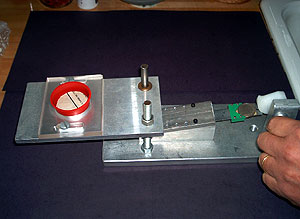
\includegraphics[width=\linewidth, height=1.5in, keepaspectratio]{../figure/coin_tosser.jpg}
\caption{A mechanical coin tosser built for Percy Diaconis by Harvard
technicians Steve Sansone and Rick Haggerty}
\label{coinfig}
\end{marginfigure}

In this chapter we focus on the second question: formally modeling
probabilistic computation and studying its power. We will show that:

\begin{enumerate}
\def\labelenumi{\arabic{enumi}.}
\item
  We can define the class \(\mathbf{BPP}\) that captures all Boolean
  functions that can be computed in polynomial time by a randomized
  algorithm. Crucially \(\mathbf{BPP}\) is still very much a \emph{worst
  case} class of computation: the probability is only over the choice of
  the random coins of the algorithm, as opposed to the choice of the
  input.
\item
  We can \emph{amplify} the success probability of randomized
  algorithms, and as a result the class \(\mathbf{BPP}\) would be
  identical if we changed the required success probability to any number
  \(p\) that lies strictly between \(1/2\) and \(1\) (and in fact any
  number in the range \(1/2 + 1/q(n)\) to \(1-2^{-q(n)}\) for any
  polynomial \(q(n)\)).
\item
  Though, as is the case for \(\mathbf{P}\) and \(\mathbf{NP}\), there
  is much we do not know about the class \(\mathbf{BPP}\), we can
  establish some relations between \(\mathbf{BPP}\) and the other
  complexity classes we saw before. In particular we will show that
  \(\mathbf{P} \subseteq \mathbf{BPP} \subseteq \mathbf{EXP}\) and
  \(\mathbf{BPP} \subseteq \mathbf{P_{/poly}}\).
\item
  While the relation between \(\mathbf{BPP}\) and \(\mathbf{NP}\) is not
  known, we can show that if \(\mathbf{P}=\mathbf{NP}\) then
  \(\mathbf{BPP}=\mathbf{P}\).
\item
  We also show that the concept of \(\mathbf{NP}\) completeness applies
  equally well if we use randomized algorithms as our model of
  ``efficient computation''. That is, if a single \(\mathbf{NP}\)
  complete problem has a randomized polynomial-time algorithm, then all
  of \(\mathbf{NP}\) can be computed in polynomial-time by randomized
  algorithms.
\item
  Finally we will discuss the question of whether
  \(\mathbf{BPP} = \mathbf{P}\) and show some of the intriguing evidence
  that the answer might actually be \emph{``Yes''} using the concept of
  \emph{pseudorandom generators}.
\end{enumerate}

\section{Modeling randomized
computation}\label{Modeling-randomized-compu}

Modeling randomized computation is actually quite easy. We can add the
following operations to any programming language such as NAND-TM,
NAND-RAM, NAND-CIRC etc..:

\begin{code}
foo = RAND()
\end{code}

where \texttt{foo} is a variable. The result of applying this operation
is that \texttt{foo} is assigned a random bit in \(\{0,1\}\). (Every
time the \texttt{RAND} operation is invoked it returns a fresh
independent random bit.) We call the programming languages that are
augmented with this extra operation RNAND-TM, RNAND-RAM, and RNAND-CIRC
respectively.

Similarly, we can easily define randomized Turing machines as Turing
machines in which the transition function \(\delta\) gets as an extra
input (in addition to the current state and symbol read from the tape) a
bit \(b\) that in each step is chosen at random \in \(\{0,1\}\). Of
course the function can ignore this bit (and have the same output
regardless of whether \(b=0\) or \(b=1\)) and hence randomized Turing
machines generalize deterministic Turing machines.

We can use the \texttt{RAND()} operation to define the notion of a
function being computed by a randomized \(T(n)\) time algorithm for
every nice time bound \(T:\N \rightarrow \N\), as well as the notion of
a finite function being computed by a size \(S\) randomized NAND-CIRC
program (or, equivalently, a randomized circuit with \(S\) gates that
correspond to either the NAND or coin-tossing operations). However, for
simplicity we will not define randomized computation in full generality,
but simply focus on the class of functions that are computable by
randomized algorithms \emph{running in polynomial time}, which by
historical convention is known as \(\mathbf{BPP}\):

\hypertarget{BPPdef}{}
\begin{definition}[The class $\mathbf{BPP}$] \label[definition]{BPPdef}

Let \(F: \{0,1\}^*\rightarrow \{0,1\}\). We say that
\(F\in \mathbf{BPP}\) if there exist constants \(a,b\in \N\) and an
RNAND-TM program \(P\) such that for every \(x\in \{0,1\}^*\), on input
\(x\), the program \(P\) halts within at most \(a|x|^b\) steps and \[
\Pr[ P(x)= F(x)] \geq \tfrac{2}{3} \label{BPPdefinitioneq}
\] where this probability is taken over the result of the RAND
operations of \(P\).

\end{definition}

Note that the probability in \eqref{BPPdefinitioneq} is taken only over
the random choices in the execution of \(P\) and \emph{not} over the
choice of the input \(x\). In particular, as discussed in
\cref{randomworstcaseidea}, \(\mathbf{BPP}\) is still a \emph{worst
case} complexity class, in the sense that if \(F\) is in
\(\mathbf{BPP}\) then there is a polynomial-time randomized algorithm
that computes \(F\) with probability at least \(2/3\) \emph{on every
possible} (and not just random) input.

The same polynomial-overhead simulation of NAND-RAM programs by NAND-TM
programs we saw in \cref{polyRAMTM-thm} extends to \emph{randomized}
programs as well. Hence the class \(\mathbf{BPP}\) is the same
regardless of whether it is defined via RNAND-TM or RNAND-RAM programs.
Similarly, we could have just as well defined \(\mathbf{BPP}\) using
randomized Turing machines.

Because of these equivalences, below we will use the name
\emph{``polynomial time randomized algorithm''} to denote a computation
that can be modeled by a polynomial-time RNAND-TM program, RNAND-RAM
program, or a randomized Turing machine (or any programming language
that includes a coin tossing operation). Since all these models are
equivalent up to polynomial factors, you can use your favorite model to
capture polynomial-time randomized algorithms without any loss in
generality.

\hypertarget{choosingfromsetex}{}
\begin{solvedexercise}[Choosing from a set] \label[solvedexercise]{choosingfromsetex}

Modern programming languages often involve not just the ability to toss
a random coin in \(\{0,1\}\) but also to choose an element at random
from a set \(S\). Show that you can emulate this primitive using coin
tossing. Specifically, show that there is randomized algorithm \(A\)
that on input a set \(S\) of \(m\) strings of length \(n\), runs in time
\(poly(n,m)\) and outputs either an element \(x\in S\) or ``fail'' such
that

\begin{enumerate}
\def\labelenumi{\arabic{enumi}.}
\item
  Let \(p\) be the probability that \(A\) outputs ``fail'', then
  \(p < 2^{-n}\) (a number small enough that it can be ignored).
\item
  For every \(x \in S\), the probability that \(A\) outputs \(x\) is
  exactly \(\tfrac{1-p}{m}\) (and so the output is uniform over \(S\) if
  we ignore the tiny probability of failure)
\end{enumerate}

\end{solvedexercise}

\begin{solution} \label[solution]{If-the-size-of-S-is-a-pow}

If the size of \(S\) is a power of two, that is \(m=2^\ell\) for some
\(\ell\in N\), then we can choose a random element in \(S\) by tossing
\(\ell\) coins to obtain a string \(w \in \{0,1\}^\ell\) and then output
the \(i\)-th element of \(S\) where \(i\) is the number whose binary
representation is \(w\).

If \(S\) is not a power of two, then our first attempt will be to let
\(\ell = \ceil{\log m}\) and do the same, but then output the \(i\)-th
element of \(S\) if \(i \in [m]\) and output ``fail'' otherwise.
Conditioned on not outputting ``fail'', this element is distributed
uniformly in \(S\). However, in the worst case, \(2^\ell\) can be almost
\(2m\) and so the probability of fail might be close to half. To reduce
the failure probability, we can repeat the experiment above \(n\) times.
Specifically, we will use the following algorithm

\begin{algorithm}[Sample from set]
\label[algorithm]{samplefromsetalg} ~ \\ \noindent
\begin{algorithmic}[1]
\INPUT  Set $S = \{ x_0,\ldots, x_{m-1} \}$ with $x_i\in \{0,1\}^n$ for all $i\in [m]$.
\OUTPUT  Either $x\in S$ or "fail"
\STATE Let $\ell \leftarrow \lceil \log m \rceil$
\FOR{$j = 0,1,\ldots,n-1$}
   \STATE Pick $w \sim \{0,1\}^\ell$
   \STATE Let $i\in [2^\ell]$ be number whose binary representation is $w$.
   \IF{$i<m$}
     \RETURN $x_i$
   \ENDIF
\ENDFOR
\RETURN "fail"
\end{algorithmic}
\end{algorithm}

Conditioned on not failing, the output of \cref{samplefromsetalg} is
uniformly distributed in \(S\). However, since \(2^\ell < 2m\), the
probability of failure in each iteration is less than \(1/2\) and so the
probability of failure in all of them is at most \((1/2)^{n}= 2^{-n}\).

\end{solution}

\subsection{An alternative view: random coins as an ``extra
input''}\label{An-alternative-view-rando}

While we presented randomized computation as adding an extra ``coin
tossing'' operation to our programs, we can also model this as being
given an additional extra input. That is, we can think of a randomized
algorithm \(A\) as a \emph{deterministic} algorithm \(A'\) that takes
\emph{two inputs} \(x\) and \(r\) where the second input \(r\) is chosen
at random from \(\{0,1\}^m\) for some \(m\in \N\) (see
\cref{randomalgsviewsfig}). The equivalence to the \cref{BPPdef} is
shown in the following theorem:


\begin{marginfigure}
\centering
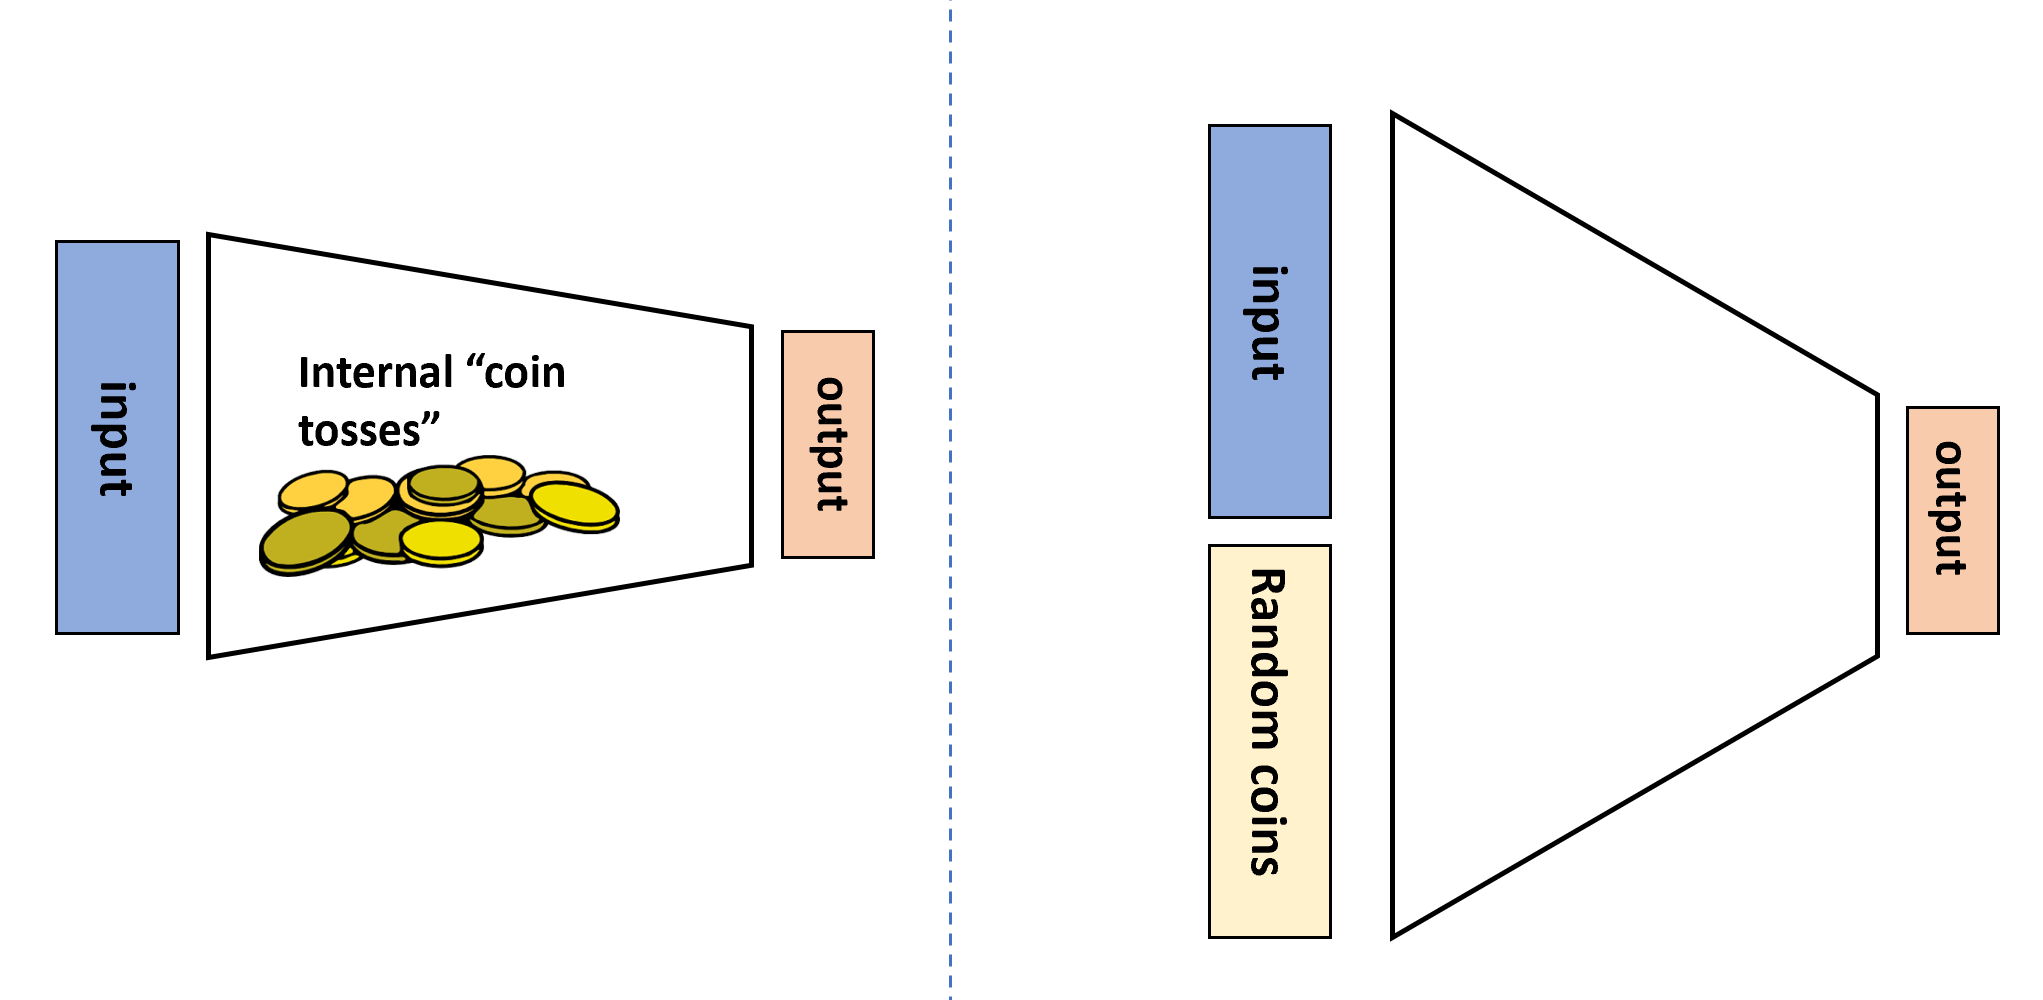
\includegraphics[width=\linewidth, height=1.5in, keepaspectratio]{../figure/randomalgstwoviews.png}
\caption{The two equivalent views of randomized algorithms. We can think
of such an algorithm as having access to an internal \texttt{RAND()}
operation that outputs a random independent value in \(\{0,1\}\)
whenever it is invoked, or we can think of it as a deterministic
algorithm that in addition to the standard input \(x \in \{0,1\}^n\)
obtains an additional auxiliary input \(r \in \{0,1\}^m\) that is chosen
uniformly at random.}
\label{randomalgsviewsfig}
\end{marginfigure}

\hypertarget{randextrainput}{}
\begin{theorem}[Alternative characterization of $\mathbf{BPP}$] \label[theorem]{randextrainput}

Let \(F:\{0,1\}^* \rightarrow \{0,1\}\). Then \(F\in \mathbf{BPP}\) if
and only if there exists \(a,b\in \N\) and
\(G:\{0,1\}^* \rightarrow \{0,1\}\) such that \(G\) is in \(\mathbf{P}\)
and for every \(x\in \{0,1\}^*\), \[
\Pr_{r\sim \{0,1\}^{a|x|^b}} [ G(xr)=F(x)] \geq \tfrac{2}{3}  \label{eqBPPauxiliary}\;.
\]

\end{theorem}

\begin{proofidea} \label[proofidea]{The-idea-behind-the-proof}

The idea behind the proof is that, as illustrated in
\cref{randomalgsviewsfig}, we can simply replace sampling a random coin
with reading a bit from the extra ``random input'' \(r\) and vice versa.
To prove this rigorously we need to work through some slightly
cumbersome formal notation. This might be one of those proofs that is
easier to work out on your own than to read.

\end{proofidea}

\begin{proof}[Proof of \cref{randextrainput}] \label[proof]{We-start-by-showing-the-o}

We start by showing the ``only if'' direction. Let \(F\in \mathbf{BPP}\)
and let \(P\) be an RNAND-TM program that computes \(F\) as per
\cref{BPPdef}, and let \(a,b\in \N\) be such that on every input of
length \(n\), the program \(P\) halts within at most \(an^b\) steps. We
will construct a polynomial-time algorithm that \(P'\) such that for
every \(x\in \{0,1\}^n\), if we set \(m=an^b\), then \[
\Pr_{r \sim \{0,1\}^{m}}[ P'(xr) = 1] = \Pr[ P(x) = 1 ] \;,
\] where the probability in the righthand side is taken over the
\texttt{RAND()} operations in \(P\). In particular this means that if we
define \(G(xr) = P'(xr)\) then the function \(G\) satisfies the
conditions of \eqref{eqBPPauxiliary}.

The algorithm \(P'\) will be very simple: it simulates the program
\(P\), maintaining a counter \(i\) initialized to \(0\). Every time that
\(P\) makes a \texttt{RAND()} operation, the program \(P'\) will supply
the result from \(r_i\) and increment \(i\) by one. We will never ``run
out'' of bits, since the running time of \(P\) is at most \(an^b\) and
hence it can make at most this number of \texttt{RNAND()} calls. The
output of \(P'(xr)\) for a random \(r\sim \{0,1\}^m\) will be
distributed identically to the output of \(P(x)\).

For the other direction, given a function \(G\in \mathbf{P}\) satisfying
the condition \eqref{eqBPPauxiliary} and a NAND-TM \(P'\) that computes
\(G\) in polynomial time, we can construct an RNAND-TM program \(P\)
that computes \(F\) in polynomial time. On input \(x\in \{0,1\}^n\), the
program \(P\) will simply use the \texttt{RNAND()} instruction \(an^b\)
times to fill an array \texttt{R[}\(0\)\texttt{]} , \(\ldots\),
\texttt{R[}\(an^b-1\)\texttt{]} and then execute the original program
\(P'\) on input \(xr\) where \(r_i\) is the \(i\)-th element of the
array \texttt{R}. Once again, it is clear that if \(P'\) runs in
polynomial time then so will \(P\), and for every input \(x\) and
\(r\in \{0,1\}^{an^b}\), the output of \(P\) on input \(x\) and where
the coin tosses outcome is \(r\) is equal to \(P'(xr)\).

\end{proof}

\hypertarget{BPPandNP}{}
\begin{remark}[Definitions of $\mathbf{BPP}$ and $\mathbf{NP}$] \label[remark]{BPPandNP}

The characterization of \(\mathbf{BPP}\) \cref{randextrainput} is
reminiscent of the characterization of \(\mathbf{NP}\) in \cref{NP-def},
with the randomness in the case of \(\mathbf{BPP}\) playing the role of
the solution in the case of \(\mathbf{NP}\). However, there are
important differences between the two:

\begin{itemize}
\item
  The definition of \(\mathbf{NP}\) is ``one sided'': \(F(x)=1\) if
  \emph{there exists} a solution \(w\) such that \(G(xw)=1\) and
  \(F(x)=0\) if \emph{for every} string \(w\) of the appropriate length,
  \(G(xw)=0\). In contrast, the characterization of \(\mathbf{BPP}\) is
  symmetric with respect to the cases \(F(x)=0\) and \(F(x)=1\).
\item
  The relation between \(\mathbf{NP}\) and \(\mathbf{BPP}\) is not
  immediately clear. It is not known whether
  \(\mathbf{BPP} \subseteq \mathbf{NP}\),
  \(\mathbf{NP} \subseteq \mathbf{BPP}\), or these two classes are
  incomparable. It is however known (with a non-trivial proof) that if
  \(\mathbf{P}=\mathbf{NP}\) then \(\mathbf{BPP}=\mathbf{P}\) (see
  \cref{BPPvsNP}).
\item
  Most importantly, the definition of \(\mathbf{NP}\) is
  ``ineffective,'' since it does not yield a way of actually finding
  whether there exists a solution among the exponentially many
  possibilities. By contrast, the definition of \(\mathbf{BPP}\) gives
  us a way to compute the function in practice by simply choosing the
  second input at random.
\end{itemize}

\end{remark}

\paragraph{Random tapes.} \cref{randextrainput} motivates sometimes
considering the randomness of an RNAND-TM (or RNAND-RAM) program as an
extra input. As such, if \(A\) is a randomized algorithm that on inputs
of length \(n\) makes at most \(m\) coin tosses, we will often use the
notation \(A(x;r)\) (where \(x\in \{0,1\}^n\) and \(r\in \{0,1\}^{m}\))
to refer to the result of executing \(x\) when the coin tosses of \(A\)
correspond to the coordinates of \(r\). This second, or ``auxiliary,''
input is sometimes referred to as a ``random tape.'' This terminology
originates from the model of randomized Turing machines.

\subsection{Success amplification of two-sided error
algorithms}\label{successamptwosided}

The number \(2/3\) might seem arbitrary, but as we've seen in
\cref{randomizedalgchap} it can be amplified to our liking:

\hypertarget{amplificationthm}{}
\begin{theorem}[Amplification] \label[theorem]{amplificationthm}

Let \(F:\{0,1\}^* \rightarrow \{0,1\}\) be a Boolean function such that
there is a polynomial \(p:\N \rightarrow \N\) and a polynomial-time
randomized algorithm \(A\) satisfying that for every \(x\in \{0,1\}^n\),
\[
\Pr[A(x) = F(x)] \geq \frac{1}{2} + \frac{1}{p(n)} \label{eqbppampassumption} \;.
\] Then for every polynomial \(q:\N \rightarrow \N\) there is a
polynomial-time randomized algorithm \(B\) satisfying for every
\(x\in \{0,1\}^n\), \[
\Pr[B(x) = F(x)] \geq  1 - 2^{-q(n)} \;.
\]

\end{theorem}

\hypertarget{amplificationidea}{}
\begin{bigidea} \label[bigidea]{amplificationidea}

We can \emph{amplify} the success of randomized algorithms to a value
that is arbitrarily close to \(1\).

\end{bigidea}

\begin{proofidea} \label[proofidea]{The-proof-is-the-same-as-}

The proof is the same as we've seen before in the case of maximum cut
and other examples. We use the Chernoff bound to argue that if \(A\)
computes \(F\) with probability at least \(\tfrac{1}{2} + \epsilon\) and
we run it \(O(k/\epsilon^2)\) times, each time using fresh and
independent random coins, then the probability that the majority of the
answers will not be correct will be less than \(2^{-k}\). Amplification
can be thought of as a ``polling'' of the choices for randomness for the
algorithm (see \cref{amplificationfig}).

\end{proofidea}

\begin{proof}[Proof of \cref{amplificationthm}] \label[proof]{Let-A-be-an-algorithm-sat}

Let \(A\) be an algorithm satisfying \eqref{eqbppampassumption}. Set
\(\epsilon = \tfrac{1}{p(n)}\) and \(k = q(n)\) where \(p,q\) are the
polynomials in the theorem statement. We can run \(P\) on input \(x\)
for \(t=10k/\epsilon^2\) times, using fresh randomness in each
execution, and compute the outputs \(y_0,\ldots,y_{t-1}\). We output the
value \(y\) that appeared the largest number of times. Let \(X_i\) be
the random variable that is equal to \(1\) if \(y_i = F(x)\) and equal
to \(0\) otherwise. The random variables \(X_0,\ldots,X_{t-1}\) are
i.i.d. and satisfy \(\E [X_i] = \Pr[ X_i = 1] \geq 1/2 + \epsilon\), and
hence by linearity of expectation
\(\mathbb{E}[\sum_{i=0}^{t-1} X_i] \geq t(1/2 + \epsilon)\). For the
plurality value to be \emph{incorrect}, it must hold that
\(\sum_{i=0}^{t-1} X_i \leq t/2\), which means that
\(\sum_{i=0}^{t-1}X_i\) is at least \(\epsilon t\) far from its
expectation. Hence by the Chernoff bound (\cref{chernoffthm}), the
probability that the plurality value is not correct is at most
\(2e^{-\epsilon^2 t}\), which is smaller than \(2^{-k}\) for our choice
of \(t\).

\end{proof}


\begin{marginfigure}
\centering
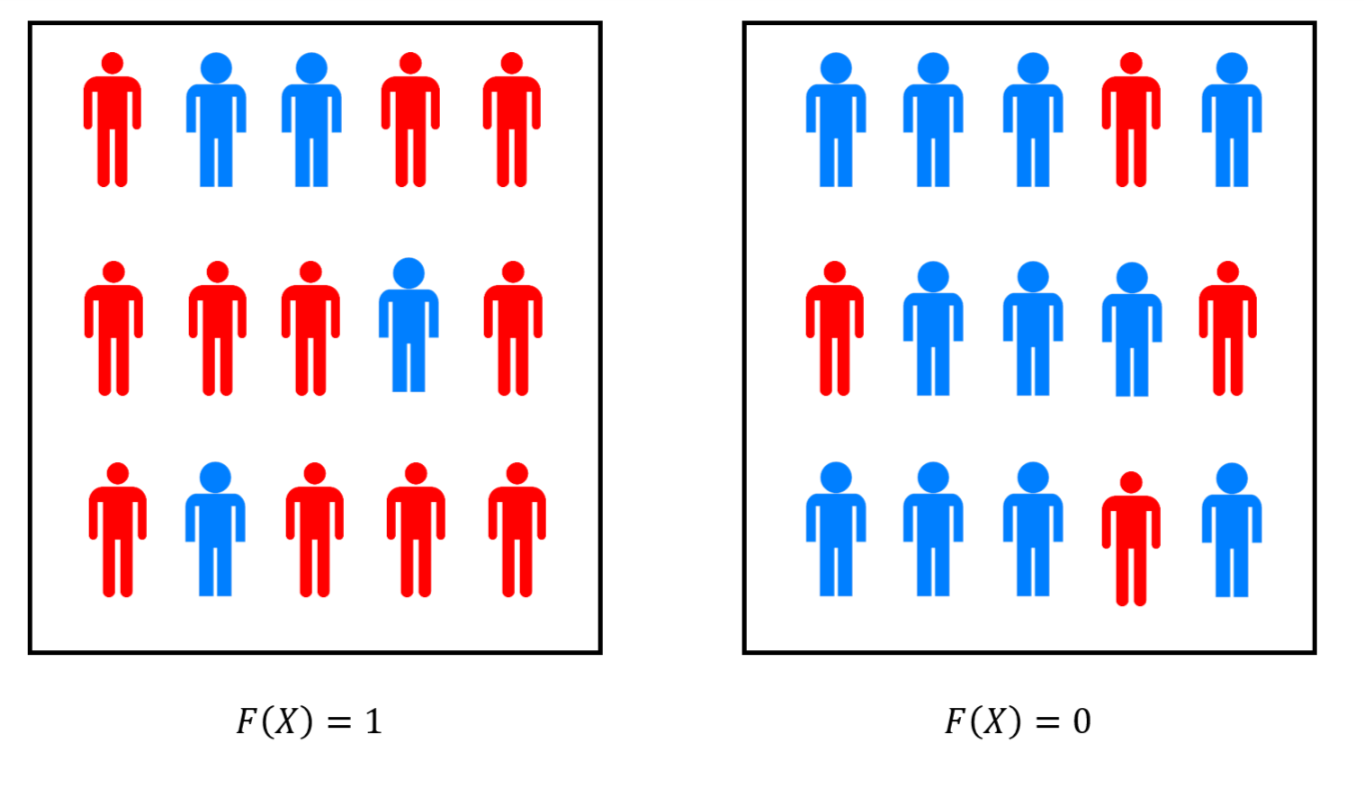
\includegraphics[width=\linewidth, height=1.5in, keepaspectratio]{../figure/BPPamplification.png}
\caption{If \(F\in\mathbf{BPP}\) then there is randomized
polynomial-time algorithm \(P\) with the following property: In the case
\(F(x)=0\) two thirds of the ``population'' of random choices satisfy
\(P(x;r)=0\) and in the case \(F(x)=1\) two thirds of the population
satisfy \(P(x;r)=1\). We can think of amplification as a form of
``polling'' of the choices of randomness. By the Chernoff bound, if we
poll a sample of \(O(\tfrac{\log(1/\delta)}{\epsilon^2})\) random
choices \(r\), then with probability at least \(1-\delta\), the fraction
of \(r\)'s in the sample satisfying \(P(x;r)=1\) will give us an
estimate of the fraction of the population within an \(\epsilon\) margin
of error. This is the same calculation used by pollsters to determine
the needed sample size in their polls.}
\label{amplificationfig}
\end{marginfigure}

\section{\(\mathbf{BPP}\) and \(\mathbf{NP}\)
completeness}\label{mathbfBPP-and-mathbfNP-co}

Since ``noisy processes'' abound in nature, randomized algorithms can be
realized physically, and so it is reasonable to propose \(\mathbf{BPP}\)
rather than \(\mathbf{P}\) as our mathematical model for ``feasible'' or
``tractable'' computation. One might wonder if this makes all the
previous chapters irrelevant, and in particular if the theory of
\(\mathbf{NP}\) completeness still applies to probabilistic algorithms.
Fortunately, the answer is \emph{Yes}:

\hypertarget{NPCandBPP}{}
\begin{theorem}[NP hardness and BPP] \label[theorem]{NPCandBPP}

Suppose that \(F\) is \(\mathbf{NP}\)-hard and \(F\in \mathbf{BPP}\).
Then \(\mathbf{NP} \subseteq \mathbf{BPP}\).

\end{theorem}

Before seeing the proof, note that \cref{NPCandBPP} implies that if
there was a randomized polynomial time algorithm for any
\(\mathbf{NP}\)-complete problem such as \(3\ensuremath{\mathit{SAT}}\),
\(\ensuremath{\mathit{ISET}}\) etc., then there would be such an
algorithm for \emph{every} problem in \(\mathbf{NP}\). Thus, regardless
of whether our model of computation is deterministic or randomized
algorithms, \(\mathbf{NP}\) complete problems retain their status as the
``hardest problems in \(\mathbf{NP}\).''

\begin{proofidea} \label[proofidea]{The-idea-is-to-simply-run}

The idea is to simply run the reduction as usual, and plug it into the
randomized algorithm instead of a deterministic one. It would be an
excellent exercise, and a way to reinforce the definitions of
\(\mathbf{NP}\)-hardness and randomized algorithms, for you to work out
the proof for yourself. However for the sake of completeness, we include
this proof below.

\end{proofidea}

\begin{proof}[Proof of \cref{NPCandBPP}] \label[proof]{Suppose-that-F-is-mathbfN}

Suppose that \(F\) is \(\mathbf{NP}\)-hard and \(F\in \mathbf{BPP}\). We
will now show that this implies that
\(\mathbf{NP} \subseteq \mathbf{BPP}\). Let \(G \in \mathbf{NP}\). By
the definition of \(\mathbf{NP}\)-hardness, it follows that
\(G \leq_p F\), or that in other words there exists a polynomial-time
computable function \(R:\{0,1\}^* \rightarrow \{0,1\}^*\) such that
\(G(x)=F(R(x))\) for every \(x\in \{0,1\}^*\). Now if \(F\) is in
\(\mathbf{BPP}\) then there is a polynomial-time RNAND-TM program \(P\)
such that \[
\Pr[ P(y)= F(y) ] \geq 2/3 \label{FinBPPeq}
\] for \emph{every} \(y\in \{0,1\}^*\) (where the probability is taken
over the random coin tosses of \(P\)). Hence we can get a
polynomial-time RNAND-TM program \(P'\) to compute \(G\) by setting
\(P'(x)=P(R(x))\). By \eqref{FinBPPeq}
\(\Pr[ P'(x) = F(R(x))] \geq 2/3\) and since \(F(R(x))=G(x)\) this
implies that \(\Pr[ P'(x) = G(x)] \geq 2/3\), which proves that
\(G \in \mathbf{BPP}\).

\end{proof}

Most of the results we've seen about \(\mathbf{NP}\) hardness, including
the search to decision reduction of \cref{search-dec-thm}, the decision
to optimization reduction of \cref{optimizationnp}, and the quantifier
elimination result of \cref{PH-collapse-thm}, all carry over in the same
way if we replace \(\mathbf{P}\) with \(\mathbf{BPP}\) as our model of
efficient computation. Thus if \(\mathbf{NP} \subseteq \mathbf{BPP}\)
then we get essentially all of the strange and wonderful consequences of
\(\mathbf{P}=\mathbf{NP}\). Unsurprisingly, we cannot rule out this
possibility. In fact, unlike \(\mathbf{P}=\mathbf{EXP}\), which is ruled
out by the time hierarchy theorem, we don't even know how to rule out
the possibility that \(\mathbf{BPP}=\mathbf{EXP}\)! Thus a priori it's
possible (though seems highly unlikely) that randomness is a magical
tool that allows us to speed up arbitrary exponential time
computation.\footnote{At the time of this writing, the largest
  ``natural'' complexity class which we can't rule out being contained
  in \(\mathbf{BPP}\) is the class \(\mathbf{NEXP}\), which we did not
  define in this course, but corresponds to non deterministic
  exponential time. See
  \href{https://people.csail.mit.edu/rrw/nexp-v-bpp.pdf}{this paper} for
  a discussion of this question.} Nevertheless, as we discuss below, it
is believed that randomization's power is much weaker and
\(\mathbf{BPP}\) lies in much more ``pedestrian'' territory.

\section{The power of randomization}\label{The-power-of-randomizatio}

A major question is whether randomization can add power to computation.
Mathematically, we can phrase this as the following question: does
\(\mathbf{BPP}=\mathbf{P}\)? Given what we've seen so far about the
relations of other complexity classes such as \(\mathbf{P}\) and
\(\mathbf{NP}\), or \(\mathbf{NP}\) and \(\mathbf{EXP}\), one might
guess that:

\begin{enumerate}
\def\labelenumi{\arabic{enumi}.}
\item
  We do not know the answer to this question.
\item
  But we suspect that \(\mathbf{BPP}\) is different than \(\mathbf{P}\).
\end{enumerate}

One would be correct about the former, but wrong about the latter. As we
will see, we do in fact have reasons to believe that
\(\mathbf{BPP}=\mathbf{P}\). This can be thought of as supporting the
\emph{extended Church Turing hypothesis} that deterministic
polynomial-time Turing machines capture what can be feasibly computed in
the physical world.

We now survey some of the relations that are known between
\(\mathbf{BPP}\) and other complexity classes we have encountered. (See
also \cref{BPPscenariosfig}.)


\begin{marginfigure}
\centering
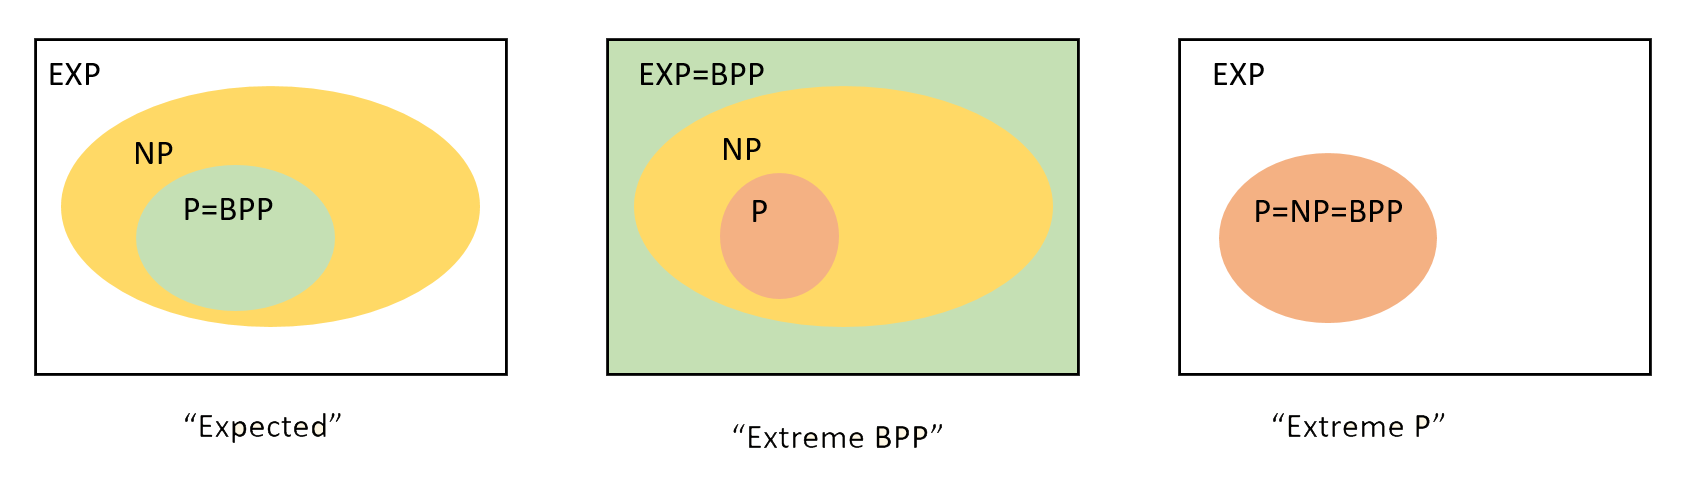
\includegraphics[width=\linewidth, height=1.5in, keepaspectratio]{../figure/BPPscenarios.png}
\caption{Some possibilities for the relations between \(\mathbf{BPP}\)
and other complexity classes. Most researchers believe that
\(\mathbf{BPP}=\mathbf{P}\) and that these classes are \emph{not}
powerful enough to solve \(\mathbf{NP}\)-complete problems, let alone
all problems in \(\mathbf{EXP}\). However, we have not even been able
yet to rule out the possibility that randomness is a ``silver bullet''
that allows exponential speedup on all problems, and hence
\(\mathbf{BPP}=\mathbf{EXP}\). As we've already seen, we also can't rule
out that \(\mathbf{P}=\mathbf{NP}\). Interestingly, in the latter case,
\(\mathbf{P}=\mathbf{BPP}\).}
\label{BPPscenariosfig}
\end{marginfigure}

\subsection{Solving \(\mathbf{BPP}\) in exponential
time}\label{Solving-mathbfBPP-in-expo}

It is not hard to see that if \(F\) is in \(\mathbf{BPP}\) then it can
be computed in \emph{exponential} time.

\hypertarget{BPPEXP}{}
\begin{theorem}[Simulating randomized algorithms in exponential time] \label[theorem]{BPPEXP}

\(\mathbf{BPP} \subseteq \mathbf{EXP}\)

\end{theorem}

\begin{pause} \label[pause]{The-proof-of-crefBPPEXP-r}

The proof of \cref{BPPEXP} readily follows by enumerating over all the
(exponentially many) choices for the random coins. We omit the formal
proof, as doing it by yourself is an excellent way to get comfortable
with \cref{BPPdef}.

\end{pause}

\subsection{Simulating randomized algorithms by
circuits}\label{Simulating-randomized-alg}

We have seen in \cref{non-uniform-thm} that if \(F\) is in
\(\mathbf{P}\), then there is a polynomial \(p:\N \rightarrow \N\) such
that for every \(n\), the restriction \(F_{\upharpoonright n}\) of \(F\)
to inputs \(\{0,1\}^n\) is in \(\ensuremath{\mathit{SIZE}}(p(n))\). (In
other words, that \(\mathbf{P} \subseteq \mathbf{P_{/poly}}\).) A priori
it is not at all clear that the same holds for a function in
\(\mathbf{BPP}\), but this does turn out to be the case.


\begin{marginfigure}
\centering
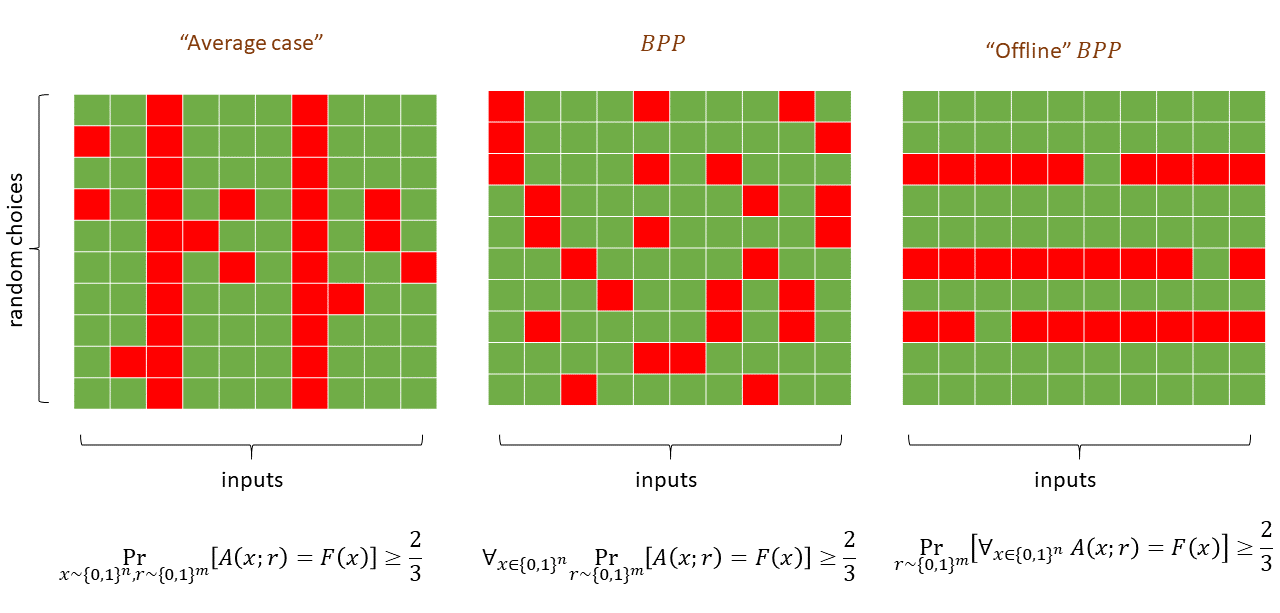
\includegraphics[width=\linewidth, height=1.5in, keepaspectratio]{../figure/randomizedcomp.png}
\caption{The possible guarantees for a randomized algorithm \(A\)
computing some function \(F\). In the tables above, the columns
correspond to different inputs and the rows to different choices of the
random tape. A cell at position \(r,x\) is colored green if
\(A(x;r)=F(x)\) (i.e., the algorithm outputs the correct answer) and red
otherwise. The standard \(\mathbf{BPP}\) guarantee corresponds to the
middle figure, where for every input \(x\), at least two thirds of the
choices \(r\) for a random tape will result in \(A\) computing the
correct value. That is, every column is colored green in at least two
thirds of its coordinates. In the left figure we have an ``average
case'' guarantee where the algorithm is only guaranteed to output the
correct answer with probability two thirds over a \emph{random} input
(i.e., at most one third of the total entries of the table are colored
red, but there could be an all red column). The right figure corresponds
to the ``offline \(\mathbf{BPP}\)'' case, with probability at least two
thirds over the random choice \(r\), \(r\) will be good for \emph{every}
input. That is, at least two thirds of the rows are all green.
\cref{rnandthm} (\(\mathbf{BPP} \subseteq \mathbf{P_{/poly}}\)) is
proven by amplifying the success of a \(\mathbf{BPP}\) algorithm until
we have the ``offline \(\mathbf{BPP}\)'' guarantee, and then hardwiring
the choice of the randomness \(r\) to obtain a nonuniform deterministic
algorithm.}
\label{randomizedcompfig}
\end{marginfigure}

\hypertarget{rnandthm}{}
\begin{theorem}[Randomness does not help for non uniform computation] \label[theorem]{rnandthm}

\(\mathbf{BPP} \subseteq \mathbf{P_{/poly}}\).

\end{theorem}

That is, for every \(F\in \mathbf{BPP}\), there exist some \(a,b\in \N\)
such that for every \(n>0\),
\(F_{\upharpoonright n} \in \ensuremath{\mathit{SIZE}}(an^b)\) where
\(F_{\upharpoonright n}\) is the restriction of \(F\) to inputs in
\(\{0,1\}^n\).

\begin{proofidea} \label[proofidea]{The-idea-behind-the-proof}

The idea behind the proof is that we can first amplify by repetition the
probability of success from \(2/3\) to \(1-0.1 \cdot 2^{-n}\). This will
allow us to show that for every \(n\in\N\) there exists a \emph{single
fixed choice} of ``favorable coins'' which is a string \(r\) of length
polynomial in \(n\) such that if \(r\) is used for the randomness then
we output the right answer on \emph{all} of the possible \(2^n\) inputs.
We can then use the standard ``unravelling the loop'' technique to
transform an RNAND-TM program to an RNAND-CIRC program, and ``hardwire''
the favorable choice of random coins to transform the RNAND-CIRC program
into a plain old deterministic NAND-CIRC program.

\end{proofidea}

\begin{proof}[Proof of \cref{rnandthm}] \label[proof]{Suppose-that-Fin-mathbfBP}

Suppose that \(F\in \mathbf{BPP}\). Let \(P\) be a polynomial-time
RNAND-TM program that computes \(F\) as per \cref{BPPdef}. Using
\cref{amplificationthm}, we can \emph{amplify} the success probability
of \(P\) to obtain an RNAND-TM program \(P'\) that is at most a factor
of \(O(n)\) slower (and hence still polynomial time) such that for every
\(x\in \{0,1\}^n\)

\[
\Pr_{r \sim \{0,1\}^m}[ P'(x;r)=F(x)] \geq 1 - 0.1\cdot 2^{-n} \;, \label{ampeq}
\]

where \(m\) is the number of coin tosses that \(P'\) uses on inputs of
length \(n\). We use the notation \(P'(x;r)\) to denote the execution of
\(P'\) on input \(x\) and when the result of the coin tosses corresponds
to the string \(r\).

For every \(x\in \{0,1\}^n\), define the ``bad'' event \(B_x\) to hold
if \(P'(x) \neq F(x)\), where the sample space for this event consists
of the coins of \(P'\). Then by \eqref{ampeq},
\(\Pr[B_x] \leq 0.1\cdot 2^{-n}\) for every \(x \in \{0,1\}^n\). Since
there are \(2^n\) many such \(x\)'s, by the union bound we see that the
probability that the \emph{union} of the events
\(\{ B_x \}_{x\in \{0,1\}^n}\) is at most \(0.1\). This means that if we
choose \(r \sim \{0,1\}^m\), then with probability at least \(0.9\) it
will be the case that for \emph{every} \(x\in \{0,1\}^n\),
\(F(x)=P'(x;r)\). (Indeed, otherwise the event \(B_x\) would hold for
some \(x\).) In particular, because of the mere fact that the the
probability of \(\cup_{x \in \{0,1\}^n} B_x\) is smaller than \(1\),
this means that \emph{there exists} a particular \(r^* \in \{0,1\}^m\)
such that

\[P'(x;r^*)=F(x) \label{hardwirecorrecteq}
\]

for every \(x\in \{0,1\}^n\).

Now let us use the standard ``unravelling the loop'' the technique and
transform \(P'\) into a NAND-CIRC program \(Q\) of polynomial in \(n\)
size, such that \(Q(xr)=P'(x;r)\) for every \(x\in \{0,1\}^n\) and
\(r \in \{0,1\}^m\). Then by ``hardwiring'' the values
\(r^*_0,\ldots,r^*_{m-1}\) in place of the last \(m\) inputs of \(Q\),
we obtain a new NAND-CIRC program \(Q_{r^*}\) that satisfies by
\eqref{hardwirecorrecteq} that \(Q_{r^*}(x)=F(x)\) for every
\(x\in \{0,1\}^n\). This demonstrates that \(F_{\upharpoonright n}\) has
a polynomial sized NAND-CIRC program, hence completing the proof of
\cref{rnandthm}.

\end{proof}

\section{Derandomization}\label{Derandomization}

The proof of \cref{rnandthm} can be summarized as follows: we can
replace a \(poly(n)\)-time algorithm that tosses coins as it runs with
an algorithm that uses a single set of coin tosses
\(r^* \in \{0,1\}^{poly(n)}\) which will be good enough for all inputs
of size \(n\). Another way to say it is that for the purposes of
computing functions, we do not need ``online'' access to random coins
and can generate a set of coins ``offline'' ahead of time, before we see
the actual input.

But this does not really help us with answering the question of whether
\(\mathbf{BPP}\) equals \(\mathbf{P}\), since we still need to find a
way to generate these ``offline'' coins in the first place. To
derandomize an RNAND-TM program we will need to come up with a
\emph{single} deterministic algorithm that will work for \emph{all input
lengths}. That is, unlike in the case of RNAND-CIRC programs, we cannot
choose for every input length \(n\) some string
\(r^* \in \{0,1\}^{poly(n)}\) to use as our random coins.

Can we derandomize randomized algorithms, or does randomness add an
inherent extra power for computation? This is a fundamentally
interesting question but is also of practical significance. Ever since
people started to use randomized algorithms during the Manhattan
project, they have been trying to remove the need for randomness and
replace it with numbers that are selected through some deterministic
process. Throughout the years this approach has often been used
successfully, though there have been a number of failures as
well.\footnote{One amusing anecdote is a
  \href{https://www.wired.com/2017/02/russians-engineer-brilliant-slot-machine-cheat-casinos-no-fix/}{recent
  case} where scammers managed to predict the imperfect ``pseudorandom
  generator'' used by slot machines to cheat casinos. Unfortunately we
  don't know the details of how they did it, since the case was
  \href{https://www.plainsite.org/dockets/2j3mlaig6/missouri-eastern-district-court/usa-v-bliev-et-al/}{sealed}.}

A common approach people used over the years was to replace the random
coins of the algorithm by a ``randomish looking'' string that they
generated through some arithmetic progress. For example, one can use the
digits of \(\pi\) for the random tape. Using these type of methods
corresponds to what von Neumann referred to as a ``state of sin''.
(Though this is a sin that he himself frequently committed, as
generating true randomness in sufficient quantity was and still is often
too expensive.) The reason that this is considered a ``sin'' is that
such a procedure will not work in general. For example, it is easy to
modify any probabilistic algorithm \(A\) such as the ones we have seen
in \cref{randomizedalgchap}, to an algorithm \(A'\) that is
\emph{guaranteed to fail} if the random tape happens to equal the digits
of \(\pi\). This means that the procedure ``replace the random tape by
the digits of \(\pi\)'' does not yield a \emph{general} way to transform
a probabilistic algorithm to a deterministic one that will solve the
same problem. Of course, this procedure does not \emph{always} fail, but
we have no good way to determine when it fails and when it succeeds.
This reasoning is not specific to \(\pi\) and holds for every
deterministically produced string, whether it obtained by \(\pi\),
\(e\), the Fibonacci series, or anything else.

An algorithm that checks if its random tape is equal to \(\pi\) and then
fails seems to be quite silly, but this is but the ``tip of the
iceberg'' for a very serious issue. Time and again people have learned
the hard way that one needs to be very careful about producing random
bits using deterministic means. As we will see when we discuss
cryptography, many spectacular security failures and break-ins were the
result of using ``insufficiently random'' coins.

\subsection{Pseudorandom generators}\label{Pseudorandom-generators}

So, we can't use any \emph{single} string to ``derandomize'' a
probabilistic algorithm. It turns out however, that we can use a
\emph{collection} of strings to do so. Another way to think about it is
that rather than trying to \emph{eliminate} the need for randomness, we
start by focusing on \emph{reducing} the amount of randomness needed.
(Though we will see that if we reduce the randomness sufficiently, we
can eventually get rid of it altogether.)

We make the following definition:

\hypertarget{prgdef}{}
\begin{definition}[Pseudorandom generator] \label[definition]{prgdef}

A function \(G:\{0,1\}^\ell \rightarrow \{0,1\}^m\) is a
\emph{\((T,\epsilon)\)-pseudorandom generator} if for every circuit
\(C\) with \(m\) inputs, one output, and at most \(T\) gates, \[
\left| \Pr_{s\sim \{0,1\}^\ell}[C(G(s))=1] - \Pr_{r \sim \{0,1\}^m}[C(r)=1] \right| < \epsilon \label{eq:prg}
\]

\end{definition}


\begin{marginfigure}
\centering
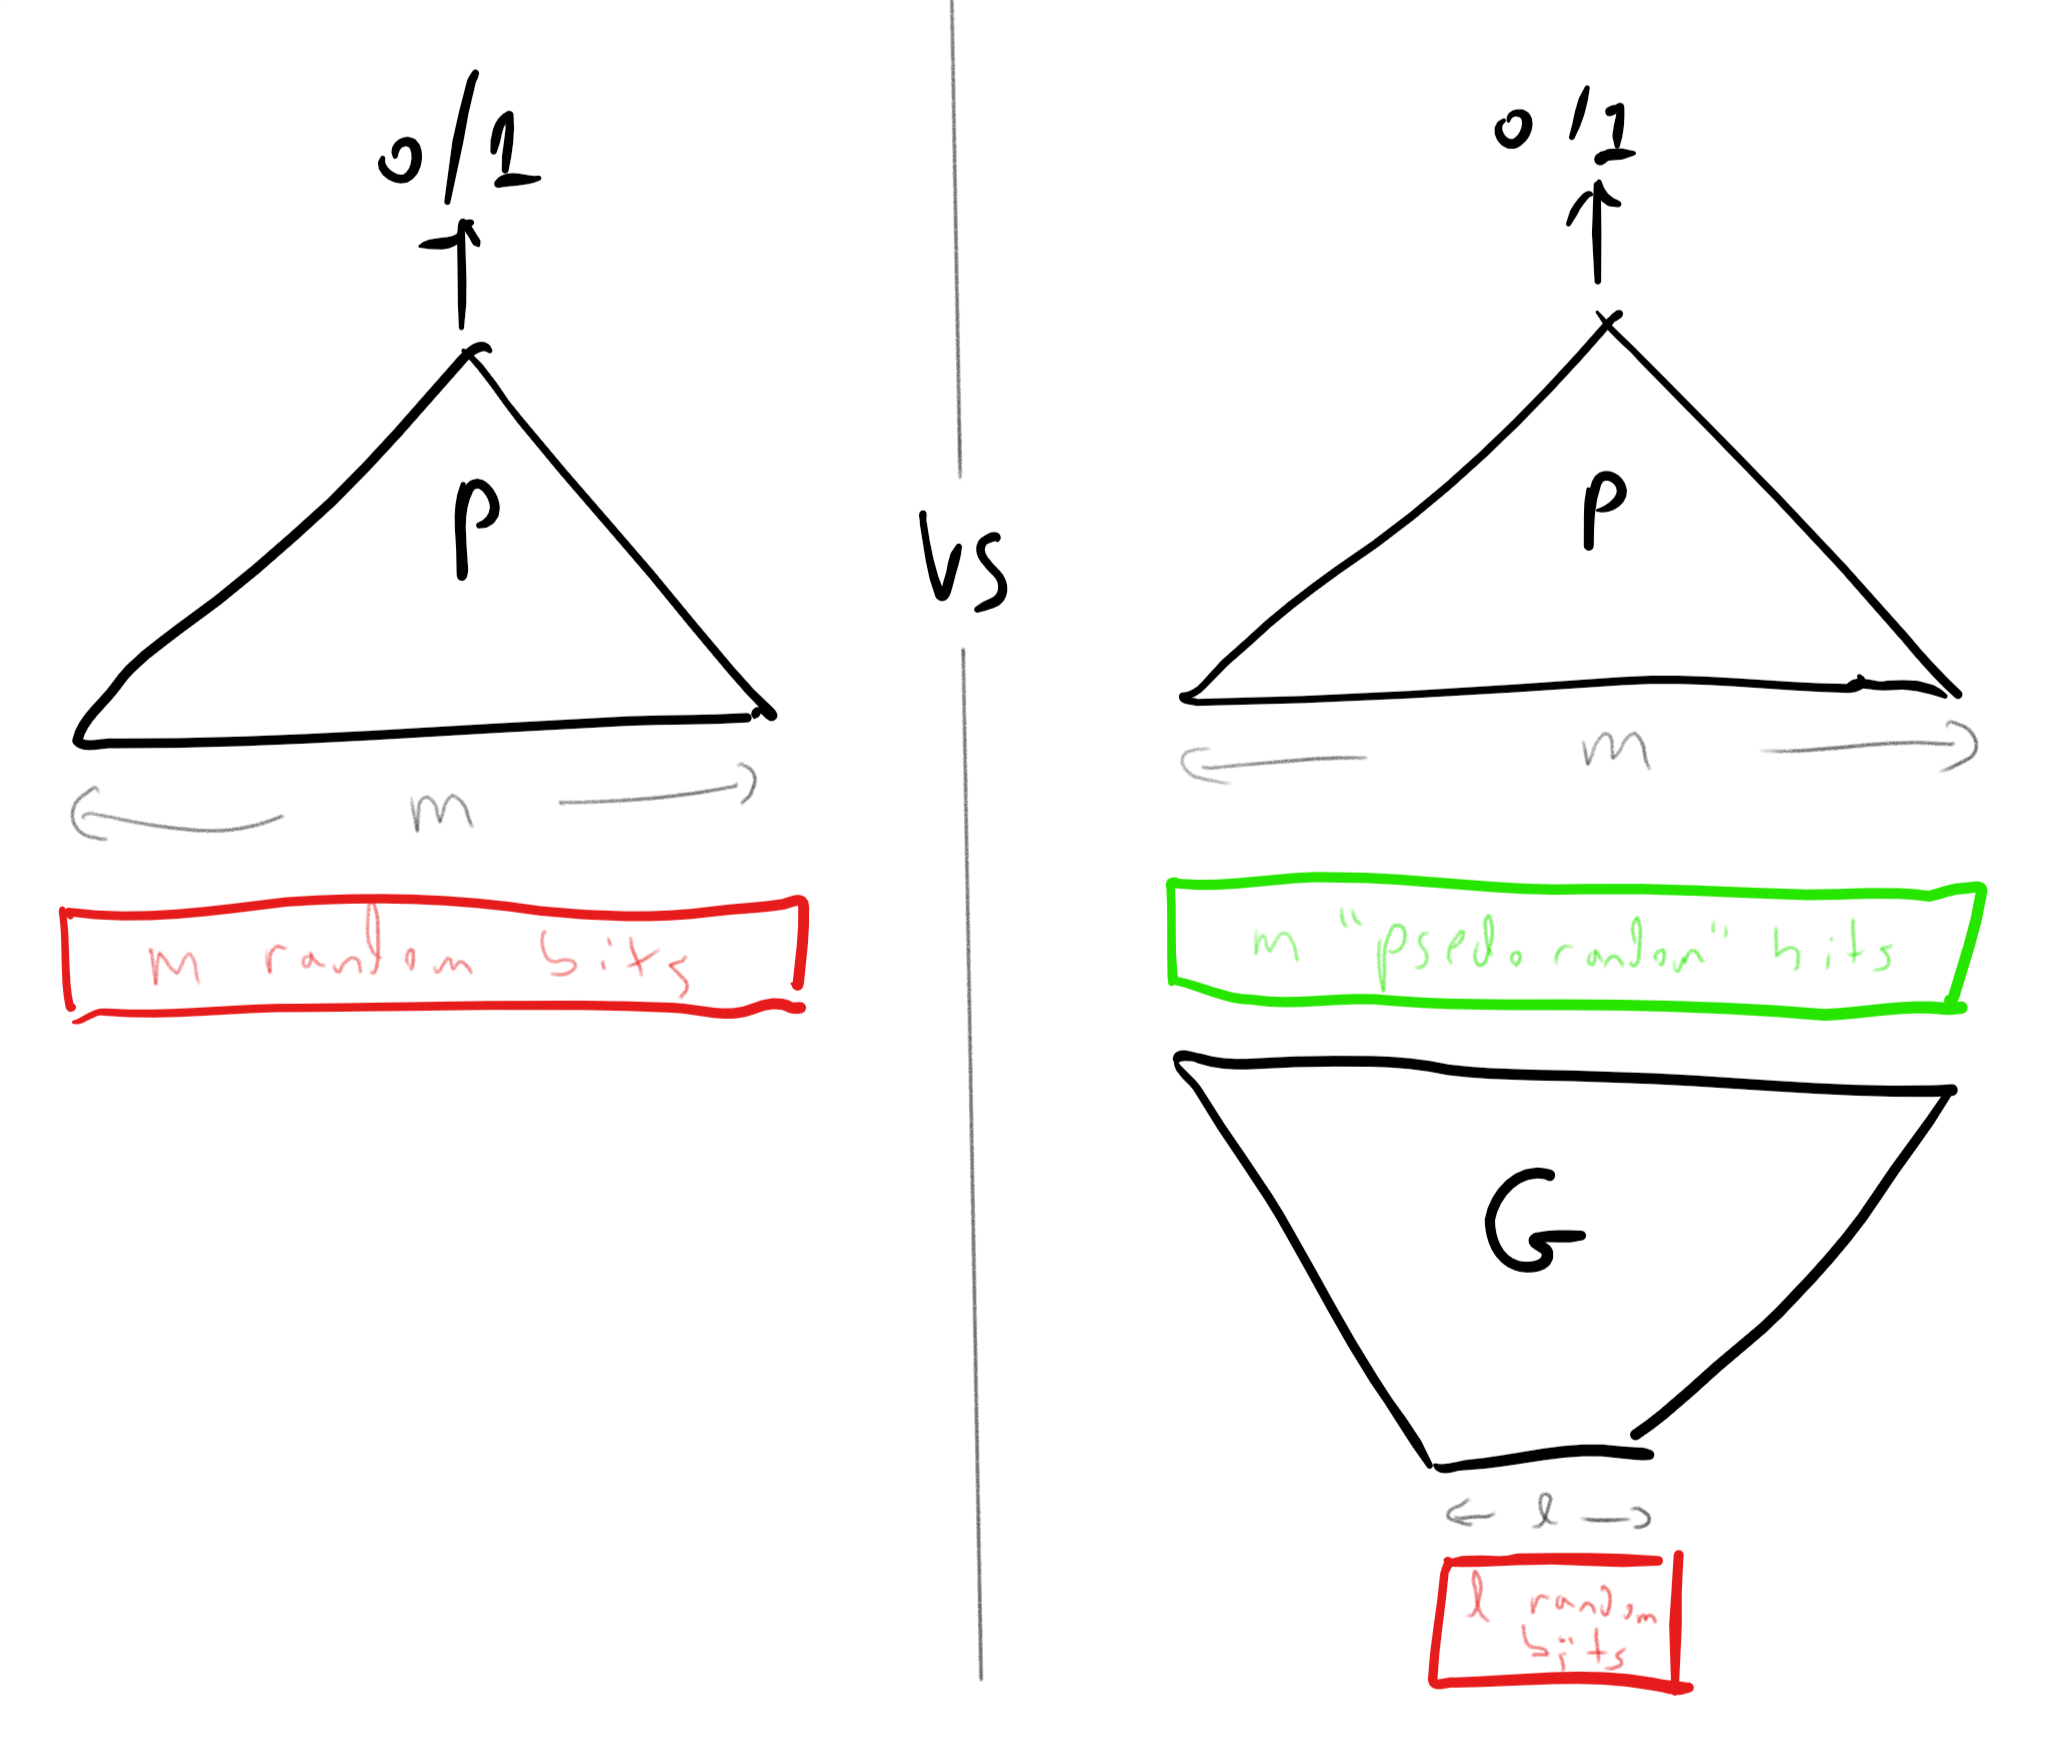
\includegraphics[width=\linewidth, height=1.5in, keepaspectratio]{../figure/prg_experiment.png}
\caption{A pseudorandom generator \(G\) maps a short string
\(s\in \{0,1\}^\ell\) into a long string \(r\in \{0,1\}^m\) such that an
small program/circuit \(P\) cannot distinguish between the case that it
is provided a random input \(r \sim \{0,1\}^m\) and the case that it is
provided a ``pseudorandom'' input of the form \(r=G(s)\) where
\(s \sim \{0,1\}^\ell\). The short string \(s\) is sometimes called the
\emph{seed} of the pseudorandom generator, as it is a small object that
can be thought as yielding a large ``tree of randomness''.}
\label{pseudorandomgeneratorfig}
\end{marginfigure}

\begin{pause} \label[pause]{This-is-a-definition-that}

This is a definition that's worth reading more than once, and spending
some time to digest it. Note that it takes several parameters:

\begin{itemize}
\item
  \(T\) is the limit on the number of gates of the circuit \(C\) that
  the generator needs to ``fool''. The larger \(T\) is, the stronger the
  generator.
\item
  \(\epsilon\) is how close is the output of the pseudorandom generator
  to the true uniform distribution over \(\{0,1\}^m\). The smaller
  \(\epsilon\) is, the stronger the generator.
\item
  \(\ell\) is the input length and \(m\) is the output length. If
  \(\ell \geq m\) then it is trivial to come up with such a generator:
  on input \(s\in \{0,1\}^\ell\), we can output \(s_0,\ldots,s_{m-1}\).
  In this case \(\Pr_{s\sim \{0,1\}^\ell}[ P(G(s))=1]\) will simply
  equal \(\Pr_{r\in \{0,1\}^m}[ P(r)=1]\), no matter how many lines
  \(P\) has. So, the smaller \(\ell\) is and the larger \(m\) is, the
  stronger the generator, and to get anything non-trivial, we need
  \(m>\ell\).
\end{itemize}

Furthermore note that although our eventual goal is to fool
probabilistic randomized algorithms that take an unbounded number of
inputs, \cref{prgdef} refers to \emph{finite} and \emph{deterministic}
NAND-CIRC programs.

\end{pause}

We can think of a pseudorandom generator as a ``randomness amplifier.''
It takes an input \(s\) of \(\ell\) bits chosen at random and expands
these \(\ell\) bits into an output \(r\) of \(m>\ell\)
\emph{pseudorandom} bits. If \(\epsilon\) is small enough then the
pseudorandom bits will ``look random'' to any NAND-CIRC program that is
not too big. Still, there are two questions we haven't answered:

\begin{itemize}
\item
  \emph{What reason do we have to believe that pseudorandom generators
  with non-trivial parameters exist?}
\item
  \emph{Even if they do exist, why would such generators be useful to
  derandomize randomized algorithms?} After all, \cref{prgdef} does not
  involve RNAND-TM or RNAND-RAM programs, but rather deterministic
  NAND-CIRC programs with no randomness and no loops.
\end{itemize}

We will now (partially) answer both questions. For the first question,
let us come clean and confess we do not know how to \emph{prove} that
interesting pseudorandom generators exist. By \emph{interesting} we mean
pseudorandom generators that satisfy that \(\epsilon\) is some small
constant (say \(\epsilon<1/3\)), \(m>\ell\), and the function \(G\)
itself can be computed in \(poly(m)\) time. Nevertheless,
\cref{prgexist} (whose statement and proof is deferred to the end of
this chapter) shows that if we only drop the last condition
(polynomial-time computability), then there do in fact exist
pseudorandom generators where \(m\) is \emph{exponentially larger} than
\(\ell\).

\begin{pause} \label[pause]{At-this-point-you-might-w}

At this point you might want to skip ahead and look at the
\emph{statement} of \cref{prgexist}. However, since its \emph{proof} is
somewhat subtle, I recommend you defer reading it until you've finished
reading the rest of this chapter.

\end{pause}

\subsection{From existence to constructivity}\label{optimalprgconj}

The fact that there \emph{exists} a pseudorandom generator does not mean
that there is one that can be efficiently computed. However, it turns
out that we can turn complexity ``on its head'' and use the assumed
\emph{non existence} of fast algorithms for problems such as 3SAT to
obtain pseudorandom generators that can then be used to transform
randomized algorithms into deterministic ones. This is known as the
\emph{Hardness vs Randomness} paradigm. A number of results along those
lines, most of which are outside the scope of this course, have led
researchers to believe the following conjecture:

\begin{quote} \label[quote]{Optimal-PRG-conjecture-Th}

\textbf{Optimal PRG conjecture:} There is a polynomial-time computable
function \(\ensuremath{\mathit{PRG}}:\{0,1\}^* \rightarrow \{0,1\}\)
that yields an \emph{exponentially secure pseudorandom generator}.

Specifically, there exists a constant \(\delta >0\) such that for every
\(\ell\) and \(m < 2^{\delta \ell}\), if we define
\(G:\{0,1\}^\ell \rightarrow \{0,1\}^m\) as
\(G(s)_i = \ensuremath{\mathit{PRG}}(s,i)\) for every
\(s\in \{0,1\}^\ell\) and \(i \in [m]\), then \(G\) is a
\((2^{\delta \ell},2^{-\delta \ell})\) pseudorandom generator.

\end{quote}

\begin{pause} \label[pause]{The-optimal-PRG-conjectur}

The ``optimal PRG conjecture'' is worth while reading more than once.
What it posits is that we can obtain \((T,\epsilon)\) pseudorandom
generator \(G\) such that every output bit of \(G\) can be computed in
time polynomial in the length \(\ell\) of the input, where \(T\) is
exponentially large in \(\ell\) and \(\epsilon\) is exponentially small
in \(\ell\). (Note that we could not hope for the entire output to be
computable in \(\ell\), as just writing the output down will take too
long.)

To understand why we call such a pseudorandom generator ``optimal,'' it
is a great exercise to convince yourself that, for example, there does
not exist a \((2^{1.1\ell},2^{-1.1\ell})\) pseudorandom generator (in
fact, the number \(\delta\) in the conjecture must be smaller than
\(1\)). To see that we can't have \(T \gg 2^{\ell}\), note that if we
allow a NAND-CIRC program with much more than \(2^\ell\) lines then this
NAND-CIRC program could ``hardwire'' inside it all the outputs of \(G\)
on all its \(2^\ell\) inputs, and use that to distinguish between a
string of the form \(G(s)\) and a uniformly chosen string in
\(\{0,1\}^m\). To see that we can't have \(\epsilon \ll 2^{-\ell}\),
note that by guessing the input \(s\) (which will be successful with
probability \(2^{-2\ell}\)), we can obtain a small (i.e., \(O(\ell)\)
line) NAND-CIRC program that achieves a \(2^{-\ell}\) advantage in
distinguishing a pseudorandom and uniform input. Working out these
details is a highly recommended exercise.

\end{pause}

We emphasize again that the optimal PRG conjecture is, as its name
implies, a \emph{conjecture}, and we still do not know how to
\emph{prove} it. In particular, it is stronger than the conjecture that
\(\mathbf{P} \neq \mathbf{NP}\). But we do have some evidence for its
truth. There is a spectrum of different types of pseudorandom
generators, and there are weaker assumptions than the optimal PRG
conjecture that suffice to prove that \(\mathbf{BPP}=\mathbf{P}\). In
particular this is known to hold under the assumption that there exists
a function \(F\in \mathbf{TIME}(2^{O(n)})\) and \(\epsilon >0\) such
that for every sufficiently large \(n\), \(F_{\upharpoonright n}\) is
not in \(\ensuremath{\mathit{SIZE}}(2^{\epsilon n})\). The name
``Optimal PRG conjecture'' is non standard. This conjecture is sometimes
known in the literature as the existence of \emph{exponentially strong
pseudorandom functions}.\footnote{A pseudorandom generator of the form
  we posit, where each output bit can be computed individually in time
  polynomial in the seed length, is commonly known as a
  \emph{pseudorandom function generator}. For more on the many
  interesting results and connections in the study of
  \emph{pseudorandomness}, see
  \href{https://people.seas.harvard.edu/~salil/pseudorandomness/}{this
  monograph of Salil Vadhan}.}

\subsection{Usefulness of pseudorandom
generators}\label{Usefulness-of-pseudorando}

We now show that optimal pseudorandom generators are indeed very useful,
by proving the following theorem:

\hypertarget{derandBPPthm}{}
\begin{theorem}[Derandomization of BPP] \label[theorem]{derandBPPthm}

Suppose that the optimal PRG conjecture is true. Then
\(\mathbf{BPP}=\mathbf{P}\).

\end{theorem}

\begin{proofidea} \label[proofidea]{The-optimal-PRG-conjectur}

The optimal PRG conjecture tells us that we can achieve
\emph{exponential expansion} of \(\ell\) truly random coins into as many
as \(2^{\delta \ell}\) ``pseudorandom coins.'' Looked at from the other
direction, it allows us to reduce the need for randomness by taking an
algorithm that uses \(m\) coins and converting it into an algorithm that
only uses \(O(\log m)\) coins. Now an algorithm of the latter type by
can be made fully deterministic by enumerating over all the
\(2^{O(\log m)}\) (which is polynomial in \(m\)) possibilities for its
random choices.

\end{proofidea}

We now proceed with the proof details.

\begin{proof}[Proof of \cref{derandBPPthm}] \label[proof]{Let-Fin-mathbfBPP-and-let}

Let \(F\in \mathbf{BPP}\) and let \(P\) be a NAND-TM program and
\(a,b,c,d\) constants such that for every \(x\in \{0,1\}^n\), \(P(x)\)
runs in at most \(c \cdot n^d\) steps and
\(\Pr_{r\sim \{0,1\}^m}[ P(x;r) = F(x) ] \geq 2/3\). By ``unrolling the
loop'' and hardwiring the input \(x\), we can obtain for every input
\(x\in \{0,1\}^n\) a NAND-CIRC program \(Q_x\) of at most, say,
\(T=10c \cdot n^d\) lines, that takes \(m\) bits of input and such that
\(Q(r)=P(x;r)\).

Now suppose that \(G:\{0,1\}^\ell \rightarrow \{0,1\}\) is a \((T,0.1)\)
pseudorandom generator. Then we could deterministically estimate the
probability \(p(x)= \Pr_{r\sim \{0,1\}^m}[ Q_x(r) = 1 ]\) up to \(0.1\)
accuracy in time \(O(T \cdot 2^\ell \cdot m \cdot cost(G))\) where
\(cost(G)\) is the time that it takes to compute a single output bit of
\(G\).

The reason is that we know that
\(\tilde{p}(x)= \Pr_{s \sim \{0,1\}^\ell}[ Q_x(G(s)) = 1]\) will give us
such an estimate for \(p(x)\), and we can compute the probability
\(\tilde{p}(x)\) by simply trying all \(2^\ell\) possibillites for
\(s\). Now, under the optimal PRG conjecture we can set
\(T = 2^{\delta \ell}\) or equivalently
\(\ell = \tfrac{1}{\delta}\log T\), and our total computation time is
polynomial in \(2^\ell = T^{1/\delta}\). Since \(T \leq 10c \cdot n^d\),
this running time will be polynomial in \(n\).

This completes the proof, since we are guaranteed that
\(\Pr_{r\sim \{0,1\}^m}[ Q_x(r) = F(x) ] \geq 2/3\), and hence
estimating the probability \(p(x)\) to within \(0.1\) accuracy is
sufficient to compute \(F(x)\).

\end{proof}

\section{\(\mathbf{P}=\mathbf{NP}\) and \(\mathbf{BPP}\) vs
\(\mathbf{P}\)}\label{mathbfPmathbfNP-and-mathb}

Two computational complexity questions that we cannot settle are:

\begin{itemize}
\item
  Is \(\mathbf{P}=\mathbf{NP}\)? Where we believe the answer is
  \emph{negative}.
\item
  Is \(\mathbf{BPP}=\mathbf{P}\)? Where we believe the answer is
  \emph{positive}.
\end{itemize}

However we can say that the ``conventional wisdom'' is correct on at
least one of these questions. Namely, if we're wrong on the first count,
then we'll be right on the second one:

\hypertarget{BPPvsNP}{}
\begin{theorem}[Sipser–Gács Theorem] \label[theorem]{BPPvsNP}

If \(\mathbf{P}=\mathbf{NP}\) then \(\mathbf{BPP}=\mathbf{P}\).

\end{theorem}

\begin{pause} \label[pause]{Before-reading-the-proof-}

Before reading the proof, it is instructive to think why this result is
not ``obvious.'' If \(\mathbf{P}=\mathbf{NP}\) then given any randomized
algorithm \(A\) and input \(x\), we will be able to figure out in
polynomial time if there is a string \(r\in \{0,1\}^m\) of random coins
for \(A\) such that \(A(xr)=1\). The problem is that even if
\(\Pr_{r\in \{0,1\}^m}[A(xr)=F(x)] \geq 0.9999\), it can still be the
case that even when \(F(x)=0\) there exists a string \(r\) such that
\(A(xr)=1\).

The proof is rather subtle. It is much more important that you
understand the \emph{statement} of the theorem than that you follow all
the details of the proof.

\end{pause}

\begin{proofidea} \label[proofidea]{The-construction-follows-}

The construction follows the ``quantifier elimination'' idea which we
have seen in \cref{PH-collapse-thm}. We will show that for every
\(F \in \mathbf{BPP}\), we can reduce the question of some input \(x\)
satisfies \(F(x)=1\) to the question of whether a formula of the form
\(\exists_{u\in \{0,1\}^m} \forall_{v \in \{0,1\}^k} P(u,v)\) is true,
where \(m,k\) are polynomial in the length of \(x\) and \(P\) is
polynomial-time computable. By \cref{PH-collapse-thm}, if
\(\mathbf{P}=\mathbf{NP}\) then we can decide in polynomial time whether
such a formula is true or false.

The idea behind this construction is that using amplification we can
obtain a randomized algorithm \(A\) for computing \(F\) using \(m\)
coins such that for every \(x\in \{0,1\}^n\), if \(F(x)=0\) then the set
\(S \subseteq \{0,1\}^m\) of coins that make \(A\) output \(1\) is
extremely tiny, and if \(F(x)=1\) then it is very large. Now in the case
\(F(x)=1\), one can show that this means that there exists a small
number \(k\) of ``shifts'' \(s_0,\ldots,s_{k-1}\) such that the union of
the sets \(S \oplus s_i\) (i.e., sets of the form
\(\{ s\oplus s_i \;|\; s\in S \}\)) covers \(\{0,1\}^m\), while in the
case \(F(x)=0\) this union will always be of size at most \(k|S|\) which
is much smaller than \(2^m\). We can express the condition that there
exists \(s_0,\ldots,s_{k-1}\) such that
\(\cup_{i\in [k]} (S \oplus s_i) = \{0,1\}^m\) as a statement with a
constant number of quantifiers.

\end{proofidea}


\begin{marginfigure}
\centering
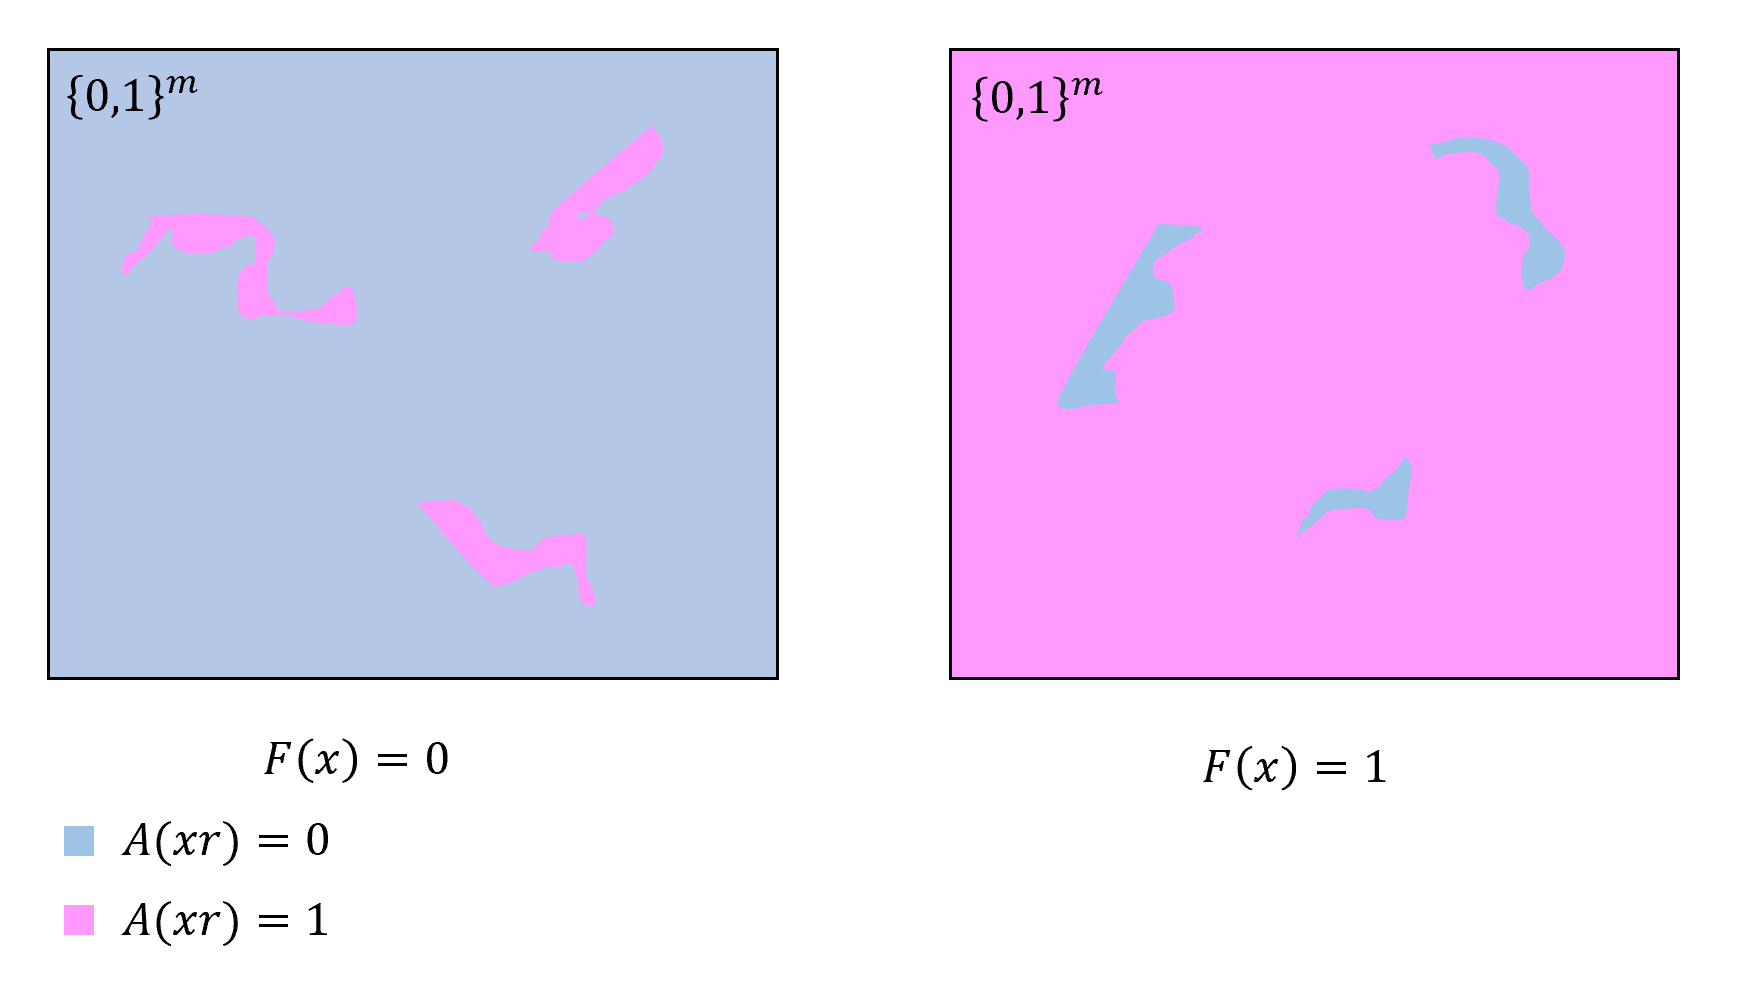
\includegraphics[width=\linewidth, height=1.5in, keepaspectratio]{../figure/strongamplification.png}
\caption{If \(F\in \mathbf{BPP}\) then through amplification we can
ensure that there is an algorithm \(A\) to compute \(F\) on \(n\)-length
inputs and using \(m\) coins such that
\(\Pr_{r\in \{0,1\}^m}[ A(xr)\neq F(x)] \ll 1/poly(m)\). Hence if
\(F(x)=1\) then almost all of the \(2^m\) choices for \(r\) will cause
\(A(xr)\) to output \(1\), while if \(F(x)=0\) then \(A(xr)=0\) for
almost all \(r\)'s. To prove the Sipser--Gács Theorem we consider
several ``shifts'' of the set \(S \subseteq \{0,1\}^m\) of the coins
\(r\) such that \(A(xr)=1\). If \(F(x)=1\) then we can find a set of
\(k\) shifts \(s_0,\ldots,s_{k-1}\) for which
\(\cup_{i\in [k]} (S \oplus s_i) = \{0,1\}^m\). If \(F(x)=0\) then for
every such set \(|cup_{i\in [k]} S_i| \leq k |S| \ll 2^m\). We can
phrase the question of whether there is such a set of shift using a
constant number of quantifiers, and so can solve it in polynomial time
if \(\mathbf{P}=\mathbf{NP}\).}
\label{strongampbppfig}
\end{marginfigure}

\begin{proof}[Proof of \cref{BPPvsNP}] \label[proof]{Let-F-in-mathbfBPP-Using-}

Let \(F \in \mathbf{BPP}\). Using \cref{amplificationthm}, there exists
a polynomial-time algorithm \(A\) such that for every
\(x\in \{0,1\}^n\),
\(\Pr_{x \in \{0,1\}^m}[ A(xr)=F(x)] \geq 1 - 2^{-n}\) where \(m\) is
polynomial in \(n\). In particular (since an exponential dominates a
polynomial, and we can always assume \(n\) is sufficiently large), it
holds that \[
\Pr_{x \in \{0,1\}^m}[ A(xr)=F(x)] \geq 1 - \tfrac{1}{10m^2}  \;. \label{sipsergacseq}
\]

Let \(x\in \{0,1\}^n\), and let \(S_x \subseteq \{0,1\}^m\) be the set
\(\{ r\in \{0,1\}^m \;:\; A(xr)=1 \}\). By our assumption, if \(F(x)=0\)
then \(|S_x| \leq \tfrac{1}{10m^2}2^{m}\) and if \(F(x)=1\) then
\(|S_x| \geq (1-\tfrac{1}{10m^2})2^m\).

For a set \(S \subseteq \{0,1\}^m\) and a string \(s\in \{0,1\}^m\), we
define the set \(S \oplus s\) to be \(\{ r \oplus s \;:\; r\in S \}\)
where \(\oplus\) denotes the XOR operation. That is, \(S \oplus s\) is
the set \(S\) ``shifted'' by \(s\). Note that \(|S \oplus s| = |S|\).
(Please make sure that you see why this is true.)

The heart of the proof is the following two claims:

\textbf{CLAIM I:} For every subset \(S \subseteq \{0,1\}^m\), if
\(|S| \leq \tfrac{1}{1000m}2^m\), then for every
\(s_0,\ldots,s_{100m-1} \in \{0,1\}^m\),
\(\cup_{i\in [100m]} (S \oplus s_i) \subsetneq \{0,1\}^m\).

\textbf{CLAIM II:} For every subset \(S \subseteq \{0,1\}^m\), if
\(|S| \geq \tfrac{1}{2}2^m\) then there exist a set of string
\(s_0,\ldots,s_{100m-1}\) such that
\(\cup_{i\in [100m]} (S \oplus s_i) = \{0,1\}^m\).

CLAIM I and CLAIM II together imply the theorem. Indeed, they mean that
under our assumptions, for every \(x\in \{0,1\}^n\), \(F(x)=1\) if and
only if

\[
\exists_{s_0,\ldots, s_{100m-1} \in \{0,1\}^m} \cup_{i\in [100m]} (S_x \oplus s_i) = \{0,1\}^m
\]

which we can re-write as

\[
\exists_{s_0,\ldots, s_{100m-1} \in \{0,1\}^m} \forall_{w\in \{0,1\}^m} \Bigl( w \in (S_x \oplus s_0) \vee w \in (S_x \oplus s_1) \vee \cdots w \in (S_x \oplus s_{100m-1}) \Bigr)
\]

or equivalently

\[
\exists_{s_0,\ldots, s_{100m-1} \in \{0,1\}^m} \forall_{w\in \{0,1\}^m} \Bigl( A(x(w\oplus s_0))=1 \vee A(x(w\oplus s_1))=1 \vee \cdots \vee A(x(w\oplus s_{100m-1}))=1    \Bigr)
\]

which (since \(A\) is computable in polynomial time) is exactly the type
of statement shown in \cref{PH-collapse-thm} to be decidable in
polynomial time if \(\mathbf{P}=\mathbf{NP}\).

We see that all that is left is to prove \textbf{CLAIM I} and
\textbf{CLAIM II}. \textbf{CLAIM I} follows immediately from the fact
that

\[
\cup_{i \in [100m-1]} |S_x \oplus s_i| \leq \sum_{i=0}^{100m-1} |S_x \oplus s_i| = \sum_{i=0}^{100m -1} |S_x| = 100m|S_x| \;.
\]

To prove \textbf{CLAIM II}, we will use a technique known as the
\emph{probabilistic method} (see the proof of \cref{prgexist} for a more
extensive discussion). Note that this is a completely different use of
probability than in the theorem statement, we just use the methods of
probability to prove an \emph{existential} statement.

\textbf{Proof of CLAIM II:} Let \(S \subseteq \{0,1\}^m\) with
\(|S| \geq 0.5 \cdot 2^m\) be as in the claim's statement. Consider the
following probabilistic experiment: we choose \(100m\) random shifts
\(s_0,\ldots,s_{100m-1}\) independently at random in \(\{0,1\}^m\), and
consider the event \(\ensuremath{\mathit{GOOD}}\) that
\(\cup_{i\in [100m]}(S \oplus s_i) = \{0,1\}^m\). To prove CLAIM II it
is enough to show that \(\Pr[ \ensuremath{\mathit{GOOD}} ] > 0\), since
that means that in particular there must \emph{exist} shifts
\(s_0,\ldots,s_{100m-1}\) that satisfy this condition.

For every \(z \in \{0,1\}^m\), define the event
\(\ensuremath{\mathit{BAD}}_z\) to hold if
\(z \not\in \cup_{i\in [100m-1]}(S \oplus s_i)\). The event
\(\ensuremath{\mathit{GOOD}}\) holds if \(\ensuremath{\mathit{BAD}}_z\)
fails for every \(z\in \{0,1\}^m\), and so our goal is to prove that
\(\Pr[ \cup_{z\in \{0,1\}^m} \ensuremath{\mathit{BAD}}_z ] <1\). By the
union bound, to show this, it is enough to show that
\(\Pr[ \ensuremath{\mathit{BAD}}_z ] < 2^{-m}\) for every
\(z\in \{0,1\}^m\). Define the event \(\ensuremath{\mathit{BAD}}_z^i\)
to hold if \(z\not\in S \oplus s_i\). Since every shift \(s_i\) is
chosen independently, for every fixed \(z\) the events
\(\ensuremath{\mathit{BAD}}_z^0,\ldots,\ensuremath{\mathit{BAD}}_z^{100m-1}\)
are mutually independent,\footnote{The condition of independence here is
  subtle. It is \emph{not} the case that all of the \(2^m \times 100m\)
  events
  \(\{ \ensuremath{\mathit{BAD}}_z^i \}_{z\in \{0,1\}^m,i\in [100m]}\)
  are mutually independent. Only for a fixed \(z \in \{0,1\}^m\), the
  \(100m\) events of the form \(\ensuremath{\mathit{BAD}}_z^i\) are
  mutually independent.} and hence

\[\Pr[ \ensuremath{\mathit{BAD}}_z ] = \Pr[ \cap_{i\in [100m-1]} \ensuremath{\mathit{BAD}}_z^i ] = \prod_{i=0}^{100m-1} \Pr[\ensuremath{\mathit{BAD}}_z^i]  \label{sipsergacsprodboundeq}\;.\]

So this means that the result will follow by showing that
\(\Pr[ \ensuremath{\mathit{BAD}}_z^i ] \leq \tfrac{1}{2}\) for every
\(z\in \{0,1\}^m\) and \(i\in [100m]\) (as that would allow to bound the
righthand side of \eqref{sipsergacsprodboundeq} by \(2^{-100m}\)). In
other words, we need to show that for every \(z\in \{0,1\}^m\) and set
\(S \subseteq \{0,1\}^m\) with \(|S| \geq \tfrac{1}{2} 2^m\),

\[\Pr_{s \in \{0,1\}^m}[ z \in S \oplus s ] \geq \tfrac{1}{2}\; \label{sipsergacsprodboundtwoeq}.\]

To show this, we observe that \(z \in S \oplus s\) if and only if
\(s \in S \oplus z\) (can you see why). Hence we can rewrite the
probability on the lefthand side of \eqref{sipsergacsprodboundtwoeq} as
\(\Pr_{s\in \{0,1\}^m}[ s\in S \oplus z]\) which simply equals
\(|S \oplus z|/2^m = |S|/2^m \geq 1/2\)! This concludes the proof of
\textbf{CLAIM I} and hence of \cref{BPPvsNP}.

\end{proof}

\section{Non-constructive existence of pseudorandom generators
(advanced, optional)}\label{Non-constructive-existenc}

We now show that, if we don't insist on \emph{constructivity} of
pseudorandom generators, then we can show that there exists pseudorandom
generators with output that \emph{exponentially larger} in the input
length.

\hypertarget{prgexist}{}
\begin{lemma}[Existence of inefficient pseudorandom generators] \label[lemma]{prgexist}

There is some absolute constant \(C\) such that for every
\(\epsilon,T\), if \(\ell > C (\log T + \log (1/\epsilon))\) and
\(m \leq T\), then there is an \((T,\epsilon)\) pseudorandom generator
\(G: \{0,1\}^\ell \rightarrow \{0,1\}^m\).

\end{lemma}

\begin{proofidea} \label[proofidea]{The-proof-uses-an-extreme}

The proof uses an extremely useful technique known as the
``probabilistic method'' which is not too hard mathematically but can be
confusing at first.\footnote{There is a whole (highly recommended)
  \href{https://www.amazon.com/Probabilistic-Method-Discrete-Mathematics-Optimization/dp/1119061954/ref=dp_ob_title_bk}{book
  by Alon and Spencer} devoted to this method.} The idea is to give a
``non constructive'' proof of existence of the pseudorandom generator
\(G\) by showing that if \(G\) was chosen at random, then the
probability that it would be a valid \((T,\epsilon)\) pseudorandom
generator is positive. In particular this means that there \emph{exists}
a single \(G\) that is a valid \((T,\epsilon)\) pseudorandom generator.
The probabilistic method is just a \emph{proof technique} to demonstrate
the existence of such a function. Ultimately, our goal is to show the
existence of a \emph{deterministic} function \(G\) that satisfies the
condition.

\end{proofidea}

The above discussion might be rather abstract at this point, but would
become clearer after seeing the proof.

\begin{proof}[Proof of \cref{prgexist}] \label[proof]{Let-epsilonTellm-be-as-in}

Let \(\epsilon,T,\ell,m\) be as in the lemma's statement. We need to
show that there exists a function
\(G:\{0,1\}^\ell \rightarrow \{0,1\}^m\) that ``fools'' every \(T\) line
program \(P\) in the sense of \eqref{eq:prg}. We will show that this
follows from the following claim:

\textbf{Claim I:} For every fixed NAND-CIRC program \(P\), if we pick
\(G:\{0,1\}^\ell \rightarrow \{0,1\}^m\) \emph{at random} then the
probability that \eqref{eq:prg} is violated is at most \(2^{-T^2}\).

Before proving Claim I, let us see why it implies \cref{prgexist}. We
can identify a function \(G:\{0,1\}^\ell \rightarrow \{0,1\}^m\) with
its ``truth table'' or simply the list of evaluations on all its
possible \(2^\ell\) inputs. Since each output is an \(m\) bit string, we
can also think of \(G\) as a string in \(\{0,1\}^{m\cdot 2^\ell}\). We
define \(\mathcal{F}^m_\ell\) to be the set of all functions from
\(\{0,1\}^\ell\) to \(\{0,1\}^m\). As discussed above we can identify
\(\mathcal{F}_\ell^m\) with \(\{0,1\}^{m\cdot 2^\ell}\) and choosing a
random function \(G \sim \mathcal{F}_\ell^m\) corresponds to choosing a
random \(m\cdot 2^\ell\)-long bit string.

For every NAND-CIRC program \(P\) let \(B_P\) be the event that, if we
choose \(G\) at random from \(\mathcal{F}_\ell^m\) then \eqref{eq:prg}
is violated with respect to the program \(P\). It is important to
understand what is the sample space that the event \(B_P\) is defined
over, namely this event depends on the choice of \(G\) and so \(B_P\) is
a subset of \(\mathcal{F}_\ell^m\). An equivalent way to define the
event \(B_P\) is that it is the subset of all functions mapping
\(\{0,1\}^\ell\) to \(\{0,1\}^m\) that violate \eqref{eq:prg}, or in
other words:

\[
B_P = \left\{ G \in \mathcal{F}_\ell^m  \; \big| \; \left| \tfrac{1}{2^\ell}\sum_{s\in \{0,1\}^\ell} P(G(s)) - \tfrac{1}{2^m}\sum_{r \in \{0,1\}^m}P(r)  \right| > \epsilon  \right\} \;\; \label{eq:eventdefine}
\] (We've replaced here the probability statements in \eqref{eq:prg}
with the equivalent sums so as to reduce confusion as to what is the
sample space that \(B_P\) is defined over.)

To understand this proof it is crucial that you pause here and see how
the definition of \(B_P\) above corresponds to \eqref{eq:eventdefine}.
This may well take re-reading the above text once or twice, but it is a
good exercise at parsing probabilistic statements and learning how to
identify the \emph{sample space} that these statements correspond to.

Now, we've shown in \cref{program-count} that up to renaming variables
(which makes no difference to program's functionality) there are
\(2^{O(T\log T)}\) NAND-CIRC programs of at most \(T\) lines. Since
\(T\log T < T^2\) for sufficiently large \(T\), this means that if Claim
I is true, then by the union bound it holds that the probability of the
union of \(B_P\) over \emph{all} NAND-CIRC programs of at most \(T\)
lines is at most \(2^{O(T\log T)}2^{-T^2} < 0.1\) for sufficiently large
\(T\). What is important for us about the number \(0.1\) is that it is
smaller than \(1\). In particular this means that there \emph{exists} a
single \(G^* \in \mathcal{F}_\ell^m\) such that \(G^*\) \emph{does not}
violate \eqref{eq:prg} with respect to any NAND-CIRC program of at most
\(T\) lines, but that precisely means that \(G^*\) is a \((T,\epsilon)\)
pseudorandom generator.

Hence to conclude the proof of \cref{prgexist}, it suffices to prove
Claim I. Choosing a random \(G: \{0,1\}^\ell \rightarrow \{0,1\}^m\)
amounts to choosing \(L=2^\ell\) random strings
\(y_0,\ldots,y_{L-1} \in \{0,1\}^m\) and letting \(G(x)=y_x\)
(identifying \(\{0,1\}^\ell\) and \([L]\) via the binary
representation). This means that proving the claim amounts to showing
that for every fixed function \(P:\{0,1\}^m \rightarrow \{0,1\}\), if
\(L > 2^{C (\log T + \log \epsilon)}\) (which by setting \(C>4\), we can
ensure is larger than \(10 T^2/\epsilon^2\)) then the probability that
\[
\left| \tfrac{1}{L}\sum_{i=0}^{L-1} P(y_i)  -  \Pr_{s \sim \{0,1\}^m}[P(s)=1] \right| > \epsilon \label{eq:prgchernoff}
\] is at most \(2^{-T^2}\).

\eqref{{eq:prgchernoff}} follows directly from the Chernoff bound.
Indeed, if we let for every \(i\in [L]\) the random variable \(X_i\)
denote \(P(y_i)\), then since \(y_0,\ldots,y_{L-1}\) is chosen
independently at random, these are independently and identically
distributed random variables with mean
\(\E_{y \sim \{0,1\}^m}[P(y)]= \Pr_{y\sim \{0,1\}^m}[ P(y)=1]\) and
hence the probability that they deviate from their expectation by
\(\epsilon\) is at most \(2\cdot 2^{-\epsilon^2 L/2}\).

\end{proof}


\begin{figure}
\centering
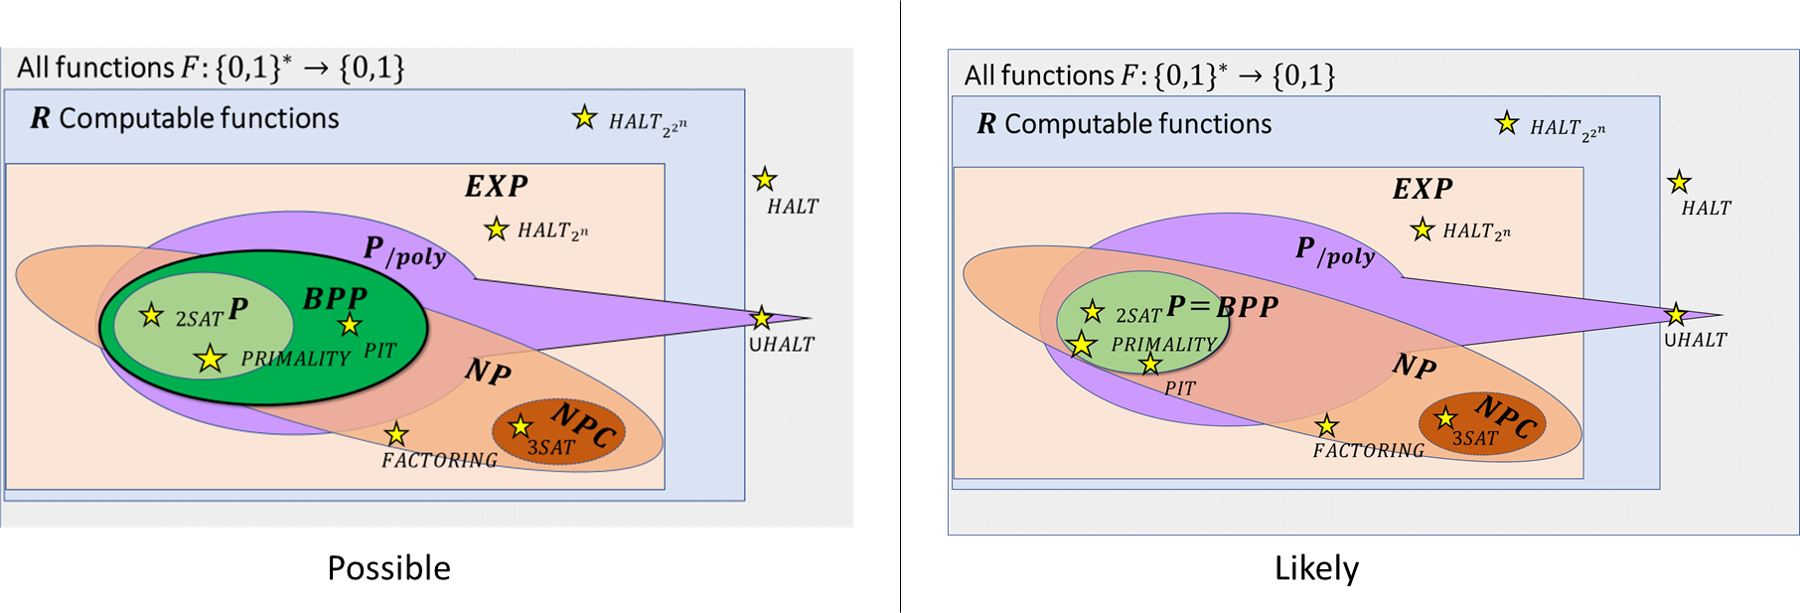
\includegraphics[width=\textwidth, height=0.25\paperheight, keepaspectratio]{../figure/bppcomplexitypicture.png}
\caption{The relation between \(\mathbf{BPP}\) and the other complexity
classes that we have seen. We know that
\(\mathbf{P} \subseteq \mathbf{BPP} \subseteq \mathbf{EXP}\) and
\(\mathbf{BPP} \subseteq \mathbf{P_{/poly}}\) but we don't know how
\(\mathbf{BPP}\) compares with \(\mathbf{NP}\) and can't rule out even
\(\mathbf{BPP} =\mathbf{EXP}\). Most evidence points out to the
possibliity that \(\mathbf{BPP}=\mathbf{P}\).}
\label{bppcomplexitypicturefig}
\end{figure}

\begin{recap} \label[recap]{We-can-model-randomized-a}

\begin{itemize}
\item
  We can model randomized algorithms by either adding a special ``coin
  toss'' operation or assuming an extra randomly chosen input.
\item
  The class \(\mathbf{BPP}\) contains the set of Boolean functions that
  can be computed by polynomial time randomized algorithms.
\item
  \(\mathbf{BPP}\) is a \emph{worst case} class of computation: a
  randomized algorithm to compute a function must compute it correctly
  with high probability \emph{on every input}.
\item
  We can \emph{amplify} the success probability of randomized algorithm
  from any value strictly larger than \(1/2\) into a success probability
  that is \emph{exponentiall close to \(1\)}.
\item
  We know that
  \(\mathbf{P} \subseteq \mathbf{BPP} \subseteq \mathbf{EXP}\).
\item
  We also know that \(\mathbf{BPP} \subseteq \mathbf{P_{/poly}}\).
\item
  The relation between \(\mathbf{BPP}\) and \(\mathbf{NP}\) is not
  known, but we do know that if \(\mathbf{P}=\mathbf{NP}\) then
  \(\mathbf{BPP}=\mathbf{P}\).
\item
  Pseudorandom generators are objects that take a short random ``seed''
  and expand it to a much longer output that ``appears random'' for
  efficient algorithms. We conjecture that exponentially strong
  pseudorandom generators exist. Under this conjecture,
  \(\mathbf{BPP}=\mathbf{P}\).
\end{itemize}

\end{recap}

\section{Exercises}\label{Exercises}

\section{Bibliographical notes}\label{modelrandbibnotes}

In this chapter we ignore the issue of how we actually get random bits
in practice. The output of many physical processes, whether it is
thermal heat, network and hard drive latency, user typing pattern and
mouse movements, and more can be thought of as a binary string sampled
from some distribution \(\mu\) that might have significant
unpredictability (or \emph{entropy}) but is not necessarily the
\emph{uniform} distribution over \(\{0,1\}^n\). Indeed, as
\href{http://statweb.stanford.edu/~susan/papers/headswithJ.pdf}{this
paper} shows, even (real-world) coin tosses do not have exactly the
distribution of a uniformly random string. Therefore, to use the
resulting measurements for randomized algorithms, one typically needs to
apply a ``distillation'' or
\href{https://en.wikipedia.org/wiki/Randomness_extractor}{randomness
extraction} process to the raw measurements to transform them to the
uniform distribution. Vadhan's book \cite{vadhan2012pseudorandomness} is
an excellent source for more discussion on both randomness extractors
and pseudorandom generators.

The name \(\mathbf{BPP}\) stands for ``bounded probability polynomial
time''. This is an historical accident: this class probably should have
been called \(\mathbf{RP}\) or \(\mathbf{PP}\) but both names were taken
by other classes.

The proof of \cref{rnandthm} actually yields more than its statement. We
can use the same ``unrolling the loop'' arguments we've used before to
show that the restriction to \(\{0,1\}^n\) of every function in
\(\mathbf{BPP}\) is also computable by a polynomial-size RNAND-CIRC
program (i.e., NAND-CIRC program with the \texttt{RAND} operation). Like
in the \(\mathbf{P}\) vs \(\ensuremath{\mathit{SIZE}}(poly(n))\) case,
there are also functions outside \(\mathbf{BPP}\) whose restrictions can
be computed by polynomial-size RNAND-CIRC programs. Nevertheless the
proof of \cref{rnandthm} shows that even such functions can be computed
by polynomial sized NAND-CIRC programs without using the \texttt{rand}
operations. This can be phrased as saying that
\(\ensuremath{\mathit{BPSIZE}}(T(n)) \subseteq \ensuremath{\mathit{SIZE}}(O(n T(n)))\)
(where \(\ensuremath{\mathit{BPSIZE}}\) is defined in the natural way
using RNAND progams). The stronger version of \cref{rnandthm} we
mentioned can be phrased as saying that
\(\mathbf{BPP_{/poly}} = \mathbf{P_{/poly}}\).
